\chapter{Model Independent Trilepton Search}\label{ch:model-independent-trilepton-search}

Events containing three or more leptons are useful probes of phenomena beyond the Standard Model. The production of three or more leptons is predicted by many models of phenomena beyond the Standard Model, as described in section~\ref{sec:beyond-the-standard-model}. The expected Standard Model backgrounds are typically small; depending on the flavor and charge of the three leptons, such events primarily arise from diboson production ($WZ$, $ZZ$), or from single boson ($W$, $Z/\gamma^{*}$) or $t\bar{t}$ production along with one or more leptons from misidentified or semileptonically decaying jets.  This dissertation presents two such searches: a model-independent search for nonresonant production of three or more leptons in many signal regions, and a signature-driven search for resonance trilepton production in the context of heavy leptons. 

This chapter presents a search for physics beyond the Standard Model using events containing three or more leptons. The search uses $20.3~\ifb$ of $pp$ collision data taken at $\sqrt{s}=8~\mbox{TeV}$ with the ATLAS detector. Many signal regions are defined based on the properties of the leptons, jets, and overall momentum imbalance of the event, with the goal of being broadly sensitive to the nonresonant production of trilepton final states by phenomena beyond the Standard Model. 

\section{Event Selection}\label{sec:model-independent-event-selection}

This section describes the selection of events containing at least three leptons in both $pp$ collision data and in the Monte Carlo simulation samples. 

\subsection{Triggering}
Collisions events for this analysis are triggered using the unprescaled single-electron or single-muon triggers with the lowest transverse momentum thresholds. At least one of the following triggers must have fired:

\begin{itemize}
	\item \texttt{ EF\_e24vhi\_medium1}: One electron with $\pt>24 \GeV$. The electron must satisfy cuts similar to the medium++ identification criteria at the trigger level, an isolation requirement of $\frac{\pt^{\mathrm{cone}20}}{\pt}<0.1$, and cuts on the leakage into the hadronic calorimeter.
	\item \texttt{ EF\_e60\_medium1}: One electron with $\pt>60 \GeV$. The electron must also satisfy the medium identification cuts, but the isolation and leakage requirements are removed.
	\item \texttt{ EF\_mu24i\_tight}: One muon with $\pt>24 \GeV$, satisfying an isolation requirement of $\frac{\pt^{\mathrm{cone}20}}{\pt}<0.12$.
	\item \texttt{ EF\_mu36\_tight}: One muon with $\pt>36 \GeV$, with no isolation requirement.
\end{itemize}

The higher-threshold triggers without isolation requirements recover efficiency at higher $\pt$. Triggered events are required to have an offline lepton matched to the trigger object within $\Delta R=\sqrt{(\Delta\eta)^2+(\Delta\phi)^2} < 0.1$. To avoid trigger turn-on effects near the $\pt$ threshold, the offline lepton must have $\pt>26 \GeV$. Additionally, trigger-matched muon must have $|\eta|<2.4$ to avoid uninstrumented regions of the detector.

%Monte Carlo events are selected using the trigger simulation. The discrepancies between the trigger performance in data and Monte Carlo are usually smaller than 2\%~\cite{Ancu:1501709}. 

\subsection{Trilepton Event Selection}\label{sec:model-independent-trilepton-event-selection}
After successful triggering and overlap removal, events are required to have at least three selected leptons, of which at most one is a hadronically decaying tau lepton. The primary event vertex, chosen as the reconstructed vertex with the highest $\sum \pt^2$ of tracks, must have at least three tracks. Finally, events are rejected if they contain ``bad jets'' not associated to real energy deposits in the calorimeters due to $pp$ collisions, i.e. from electronics problems or cosmic rays~\cite{TheATLASCollaboration:2015ds}.


\section{Analysis Strategy}\label{sec:model-independent-analysis-strategy}
The analysis defines a large number of nonexclusive signal regions, designed to target new physics models and to compartmentalize the expected backgrounds. First, the events are divided into $3\times 2$ categories as follows. First, the events are divided into three categories based on the properties of any opposite-sign, same-flavor (OSSF) lepton pairs in the event:

\begin{itemize}
	\item \textbf{on-$Z$}: events containing an opposite-sign, same-flavor lepton pair consistent with the decay of a $Z$ boson, with invariant mass within $20 \GeV$ of $m_Z$;
	\item \textbf{off-$Z$, OSSF}:  events containing an opposite-sign, same-flavor pair but vetoing on-$Z$ events; and
	\item \textbf{off-$Z$, mixed} events, containing no opposite-sign, same-flavor pairs.
\end{itemize}

The on-$Z$ category also includes events containing three leptons (two of which form a same-flavor, opposite-sign pair) with invariant mass within $20 \GeV$ of $m_Z$, to include events containing a $Z$ boson where a photon from final state radiation converts and is reconstructed as a prompt electron.

Next, the events are further divided into two categories based on the number of electron or muon candidates in the event:

\begin{itemize}
	\item \textbf{3L} events, containing at least three electrons or muons, and
	\item \textbf{2L+$\tau_{\mathrm{had}}$} events, containing exactly two electrons or muons and a hadronically decaying tau lepton.
\end{itemize}

After dividing the events into these six exclusive categories, many signal regions are defined based on the lower bound in various kinematic variables. An ordering is imposed on the leptons for the sake of disambiguation: in the 3L category, the leptons are ordered by $\pt$, while in the 2L category, the electrons or muons are ordered by $\pt$, and the $\tau_{\mathrm{had}}$ is the third lepton.  The variables used to define the signal regions are:

\begin{itemize}
	\item $\htlep$: the scalar sum of the transverse momenta of the leading three leptons. Events containing new particles with masses significantly greater than $m_W$ or $m_Z$ will typically have larger $\htlep$ than the Standard Model backgrounds.
	\item Minimum $\pt^{\ell}$: the $\pt$ of the softest of the leading three leptons. As with $\htlep$, the $\pt$ of leptons produced in the decays of heavy particles will tend to be larger than those from the expected Standard Model backgrounds.
	\item $\Htjets$: the scalar sum of the transverse momenta of all selected jets in the event. This variable is sensitive to the strong production of new physics where several leptons are produced in the decays of heavy particles, such as the gluino pair production described in section~\ref{sec:gluino-trileptons}. Conversely, the Standard Model $WZ$ and $ZZ$ backgrounds are weakly produced, and have softer $\Htjets$ distributions.
	\item $\Etmiss$: the magnitude of the missing transverse momentum in the event. In models of new physics, leptons are often produced with neutrinos in leptonic $W$ decays, or with new invisible particles, such as the stable neutralinos in many models of $R$-parity conserving SUSY. Requiring large $\Etmiss$ also suppress backgrounds due to $Z+$jets, where the jet decays semileptonically or is misidentified as a lepton. 
	\item $\meff$: the scalar sum of $\Htjets$, $\Etmiss$, and the $\pt$ of all identified leptons in the event. As with $\htlep$ by itself, multilepton production due to the decays of heavy particles will typically have a harder $\meff$ distribution than the Standard Model backgrounds.
	\item $\mtw$: for events in the on-$Z$ categories, the transverse mass of the missing transverse momentum, $\ptmiss$, and the highest-$\pt$ lepton not associated with a $Z$ boson candidate, defined as:
	\begin{equation}
		\mtw = \sqrt{2 \vec{p}_{\mathrm{T}}^{\ell}|\ptmiss|(1-\cos(\Delta\phi))},
	\end{equation}
	where $\Delta \phi$ is the azimuthal angle between the transverse momentum of the lepton, $\vec{p}_{\mathrm{T}}^{\ell}$, and the missing transverse momentum, $\ptmiss$. 
	\item $N_{b-\mathrm{tags}}$, the number of $b$-tagged jets. New physics scenarios related to the hierarchy problem (section~\ref{sec:bsm}) often couple preferentially to the third generation, due to the dominant effect of the top quark in the running of the Higgs mass. 
\end{itemize}

The signal regions are defined in table~\ref{table:model-independent-signal-regions}. The signal regions use one of $\htlep$, the minimum $\pt^{\ell}$, $\Etmiss$, $\meff$, and $n_b$ as binning variables. $\Htjets$, $\Etmiss$, and $\mtw$ are used to impose additional requirements on the signal regions. In total, 138 signal regions are defined.

\begin{table}[tbp]
  \begin{center}
    \begin{tabular}{l l r r r r l}
      \hline
      Variable     &Meaning\\
      \hline
      \Ht          &\multicolumn{6}{l}{$\Sigma\pt$ of all jets in the event}\\
      \mtw         &\multicolumn{6}{l}{Transverse mass of $W$-boson candidate (on-$Z$ events only)}\\
      \hline
      \hline
      Variable     &Meaning &\multicolumn{4}{c}{Lower Bounds [GeV]}  &Additional Requirements\\
      \hline       
      \htlep       &$\Sigma\pt$ of leading three leptons &0&200&500&800     &\\
      Min. $\ptl$  &\pt\ of softest (third) lepton       &0&50&100&150      &\\
      \met         &\multirow{2}{*}{Missing transverse momentum}       &0&100&200&300     &$\Ht < 150$ \GeV\\
      \met         &                                     &0&100&200&300     &$\Ht \geq 150$ \GeV\\
      \st          &\multirow{3}{*}{All transverse activity} &0&600&1000&1500   &\\
      \st          &                                     &0&600&1200&       &$\met{}\geq100$ \GeV\\
      \st          &                                     &0&600&1200&       &$\mtw{}\geq100$ \GeV, on-$Z$\\
      \hline
      \hline
      Variable     &Meaning &\multicolumn{4}{c}{Lower Bounds}\\
      \hline
      $b$-tags     &Number of $b$-tagged jets            &1&2&&                           &\\
      \hline
    \end{tabular}
    \caption{Kinematic signal regions defined in the analysis.}
    \label{table:model-independent-signal-regions}
  \end{center}
\end{table}


\section{Systematic Uncertainties}\label{sec:model-independent-systematics}
Systematic uncertainties are assigned to the signal and background predictions to account for possible modelling inaccuracies. The sources of uncertainty considered are:

\begin{itemize}
	\item Uncertainties on the reducible background estimates from the data-driven estimation method, as described in section~\ref{sec:fake-factor-method}. The uncertainties ranges between $20\%$ to $30\%$ for the electron fake factors, $25\%$ to $50\%$ for the muon fake factors, and $25\%$ to $30\%$ for the tau lepton fake factors.

	\item The simulated signal and background samples are normalized to the integrated luminosity of the data. The uncertainties on the normalizations are described in section~\ref{sec:prompt-background-uncertainties}. For the dominant $WZ$ and $ZZ$ backgrounds, the normalization uncertainties are $7.6\%$ and $4.3\%$, respectively.

	\item Events are also weighted to account for differences between data and Monte Carlo simulation in the lepton trigger, reconstruction, and identification efficiencies. The scale factors and associated uncertainties are provided by the relevant ATLAS combined performance groups. The electron (section~\ref{sec:reco-electron-efficiency}) and muon (section~\ref{sec:reco-muon-efficiency}) scale factors are close to unity, with uncertainties in the range $1$-$5\%$. The scale factors for the tau lepton identification efficiency range from $94$-$96\%$ for the \texttt{BDTTight} working point, and carry uncertainties between $2.0$-$2.2\%$ (section~\ref{sec:event-reconstruction-taus}).

	\item The lepton energy scales carry uncertainty which has a small effect on the signal regions due to leptons or events near $\Et$ or $\pt$ thresholds, as described in sections~\ref{sec:reco-electron-energymomentum}, \ref{sec:reco-muon-energymomentum}, and \ref{sec:reco-tau-energymomentum}.

	\item  The jet energies are scaled and smeared according to recommendations from the \texttt{JetEtMiss} combined performance group (section~\ref{sec:reco-jets-energy-scale-resolution}). The uncertainty affects the $\Htjets$ and $\meff$ distributions, and also the lepton-jet overlap removal procedure.

	\item The lepton and jet energy uncertainties are also propagated to the missing transverse energy, $\Etmiss$. 

	\item The efficiencies of the $b$-tagging algorithm carry uncertainties which are parameterized based on matching the identified $b$-jets to truth $b$-jets.

	\item Finally, the Monte Carlo samples carry statistical uncertainty due to simulating a finite number of events. 
\end{itemize}

The dominant sources of uncertainty depend on the signal region, but are generally due to Monte Carlo statistical uncertainties, the fake factor uncertainites, and theoretical cross section uncertainties. 

\section{Background Validation}\label{sec:model-independent-validation-regions}
The background estimates are verified in several dedicated validation regions, which are orthogonal to the signal regions. Events containing two leptons are used to test the selection of prompt leptons and their corresponding scale factors and energy corrections. The reducible backgrounds are tested in $t\overline{t}$ validation regions, where the events are required to have two same-sign leptons to target semileptonic decays where one lepton arises from a reducible process. Finally, the fake factor method is validated in events with modified, intermediate lepton selections, where the signal leptons are between the numerator and denominator definitions used in the nominal reducible background estimate.

\subsection{Dilepton Validation Regions}\label{sec:model-independent-validation-regions-dilepton}
Three dilepton validation regions target the three flavors of leptons: $ee$, $\mu\mu$, and $\mu\tau_{\mathrm{had}}$. The $ee$ and $\mu\mu$ regions require an opposite-sign lepton pair of the appropriate flavor. The invariant mass distributions of the dilepton system in these regions are shown in figure~\ref{fig:model-independent-VR-dilepton}. Some disagreement is observed in the $ee$ invariant mass distribution; this discrepancy is covered by the electron energy scale systematic uncertainties. 

\begin{figure}[htbp]
  \subfloat[$ee$]{
    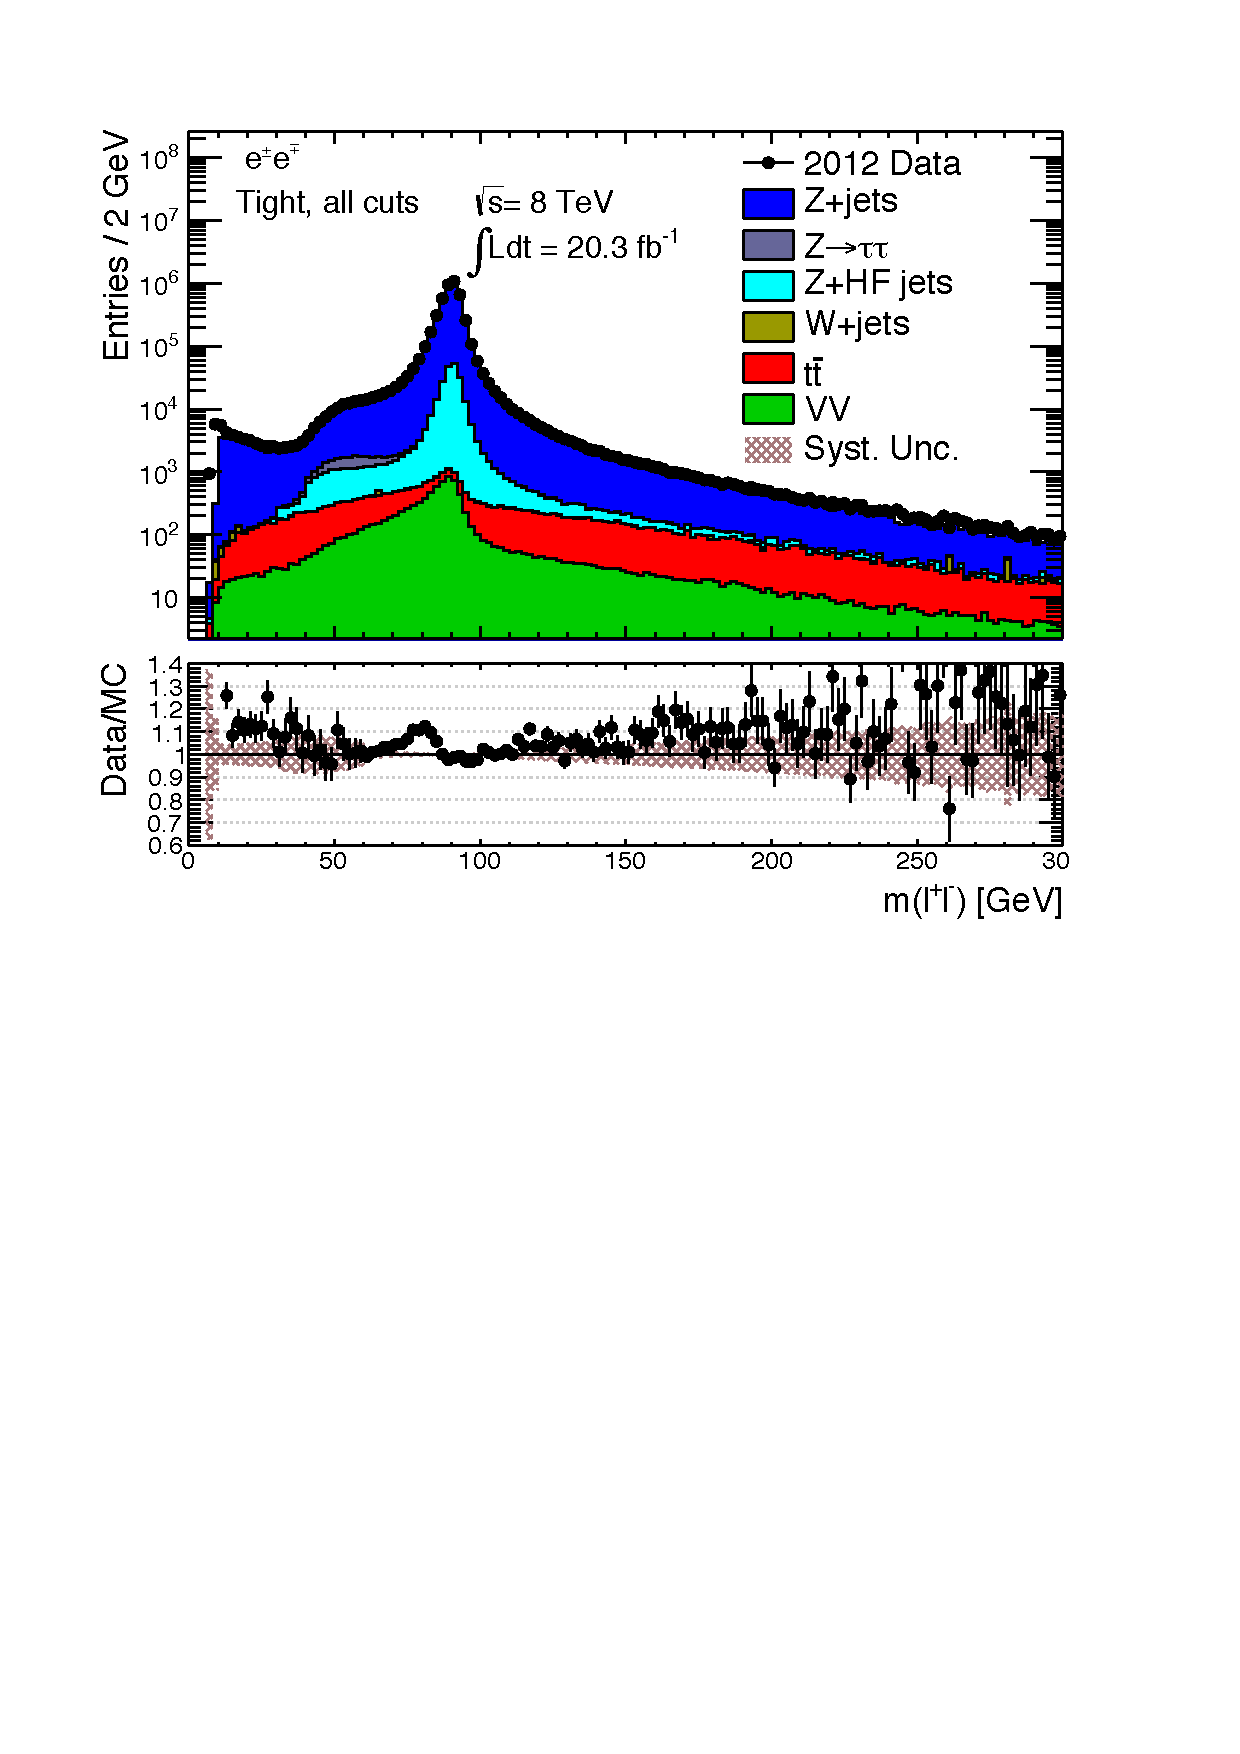
\includegraphics[width=.48\columnwidth]{figures/modelindependent/DYOSee_cut_3f_AllLeptonMass_NoLabel_Cropped}
  }
  \subfloat[$\mu\mu$]{
    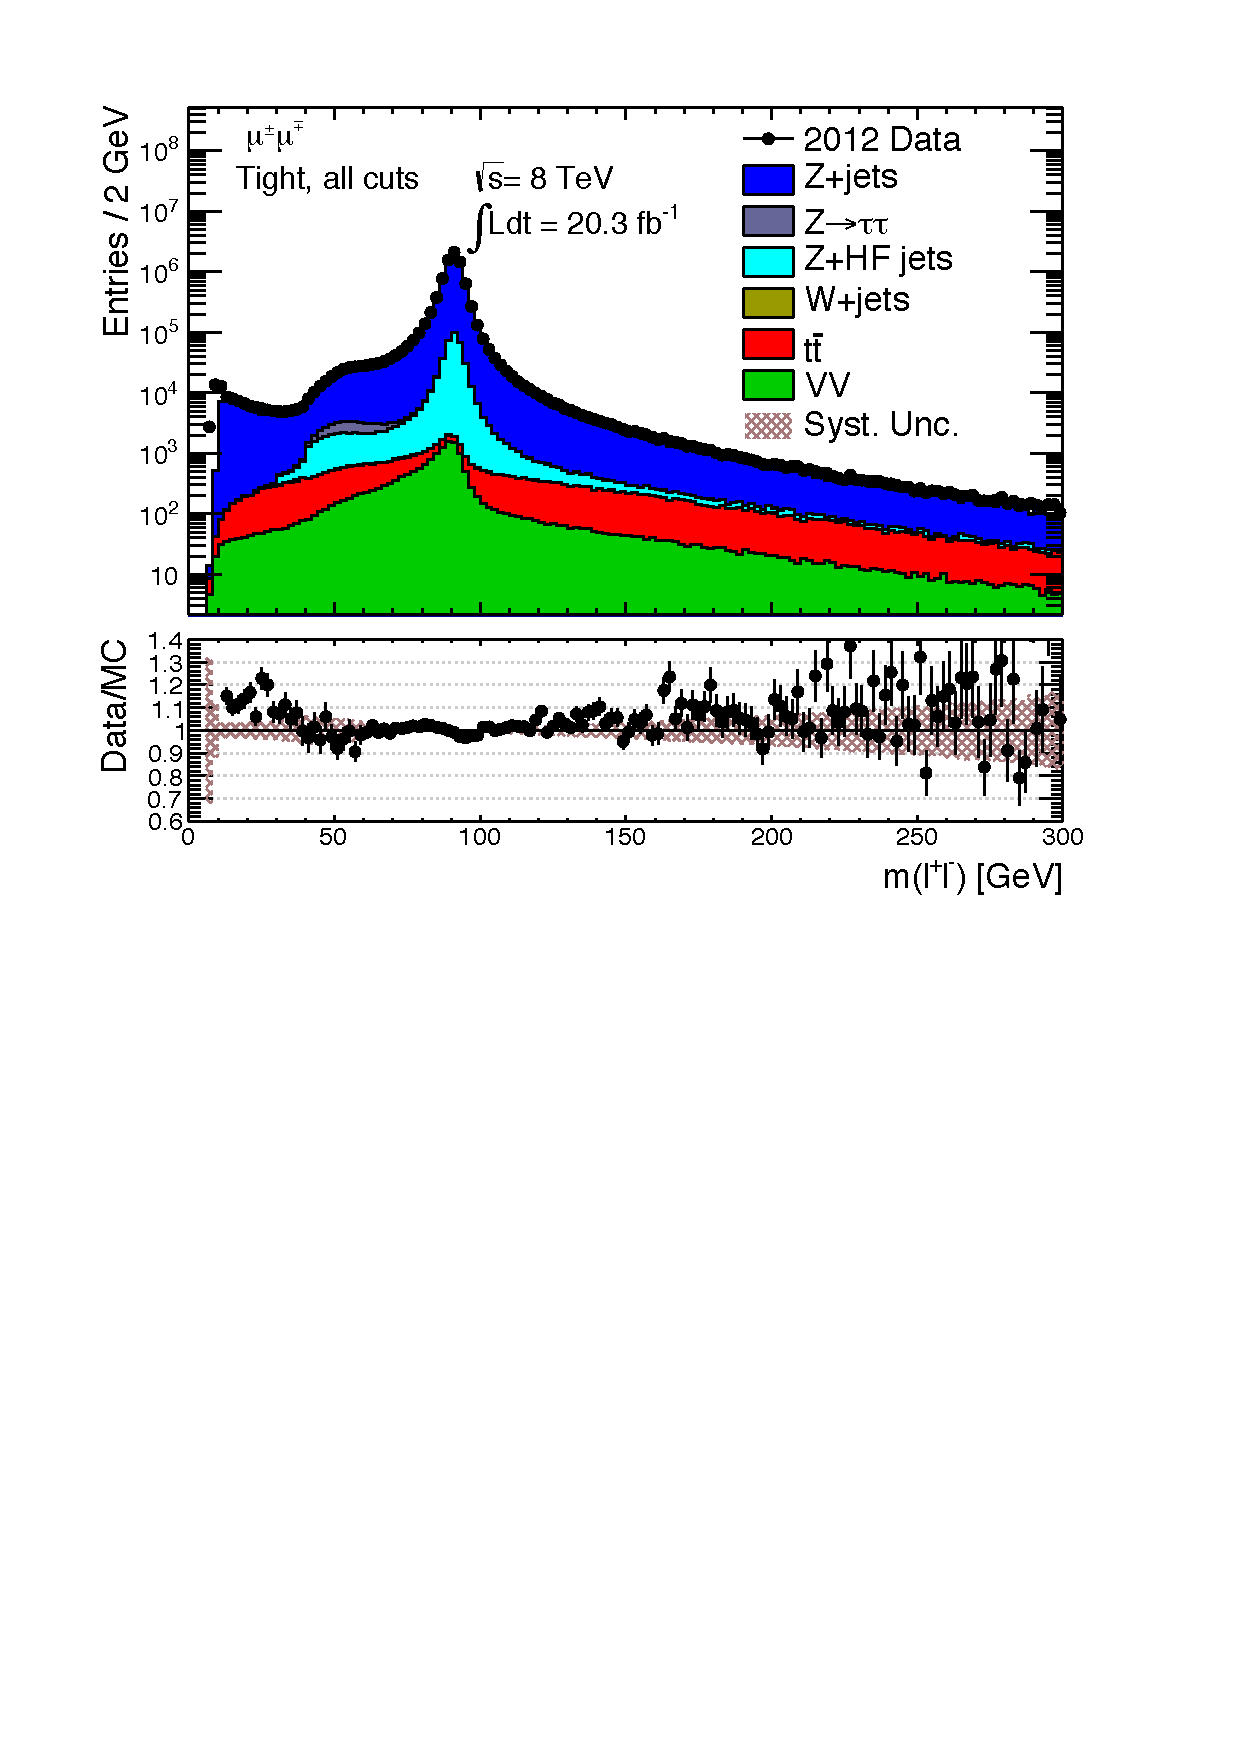
\includegraphics[width=.48\columnwidth]{figures/modelindependent/DYOSmm_cut_3f_AllLeptonMass_NoLabel_Cropped}
  }
  \caption{Dilepton invariant mass distributions for the $ee$ (left) and $\mu\mu$ (right) validation regions.}
  \label{fig:model-independent-VR-dilepton}
\end{figure}

The $ee$ and $\mu\mu$ validation regions are also used to generate scale factors to account for efficiency
differences between simulation and data when applying cuts on lepton isolation or impact parameter. The scale factors are computed from events with a dilepton pair with invariant mass within $10 \GeV$ of $m_Z$, and are shown in figure~\ref{fig:model-independent-lepton-SFs}. The scale factors are mostly consistent with unity to within $0.5\%$, except for isolation requirements on the low-$\pt$ leptons, where the scale factors deviate from unity by up to $2\%$. 

\begin{figure}[tbp]
  \subfloat[Electron \pt\ Scale Factors]{
    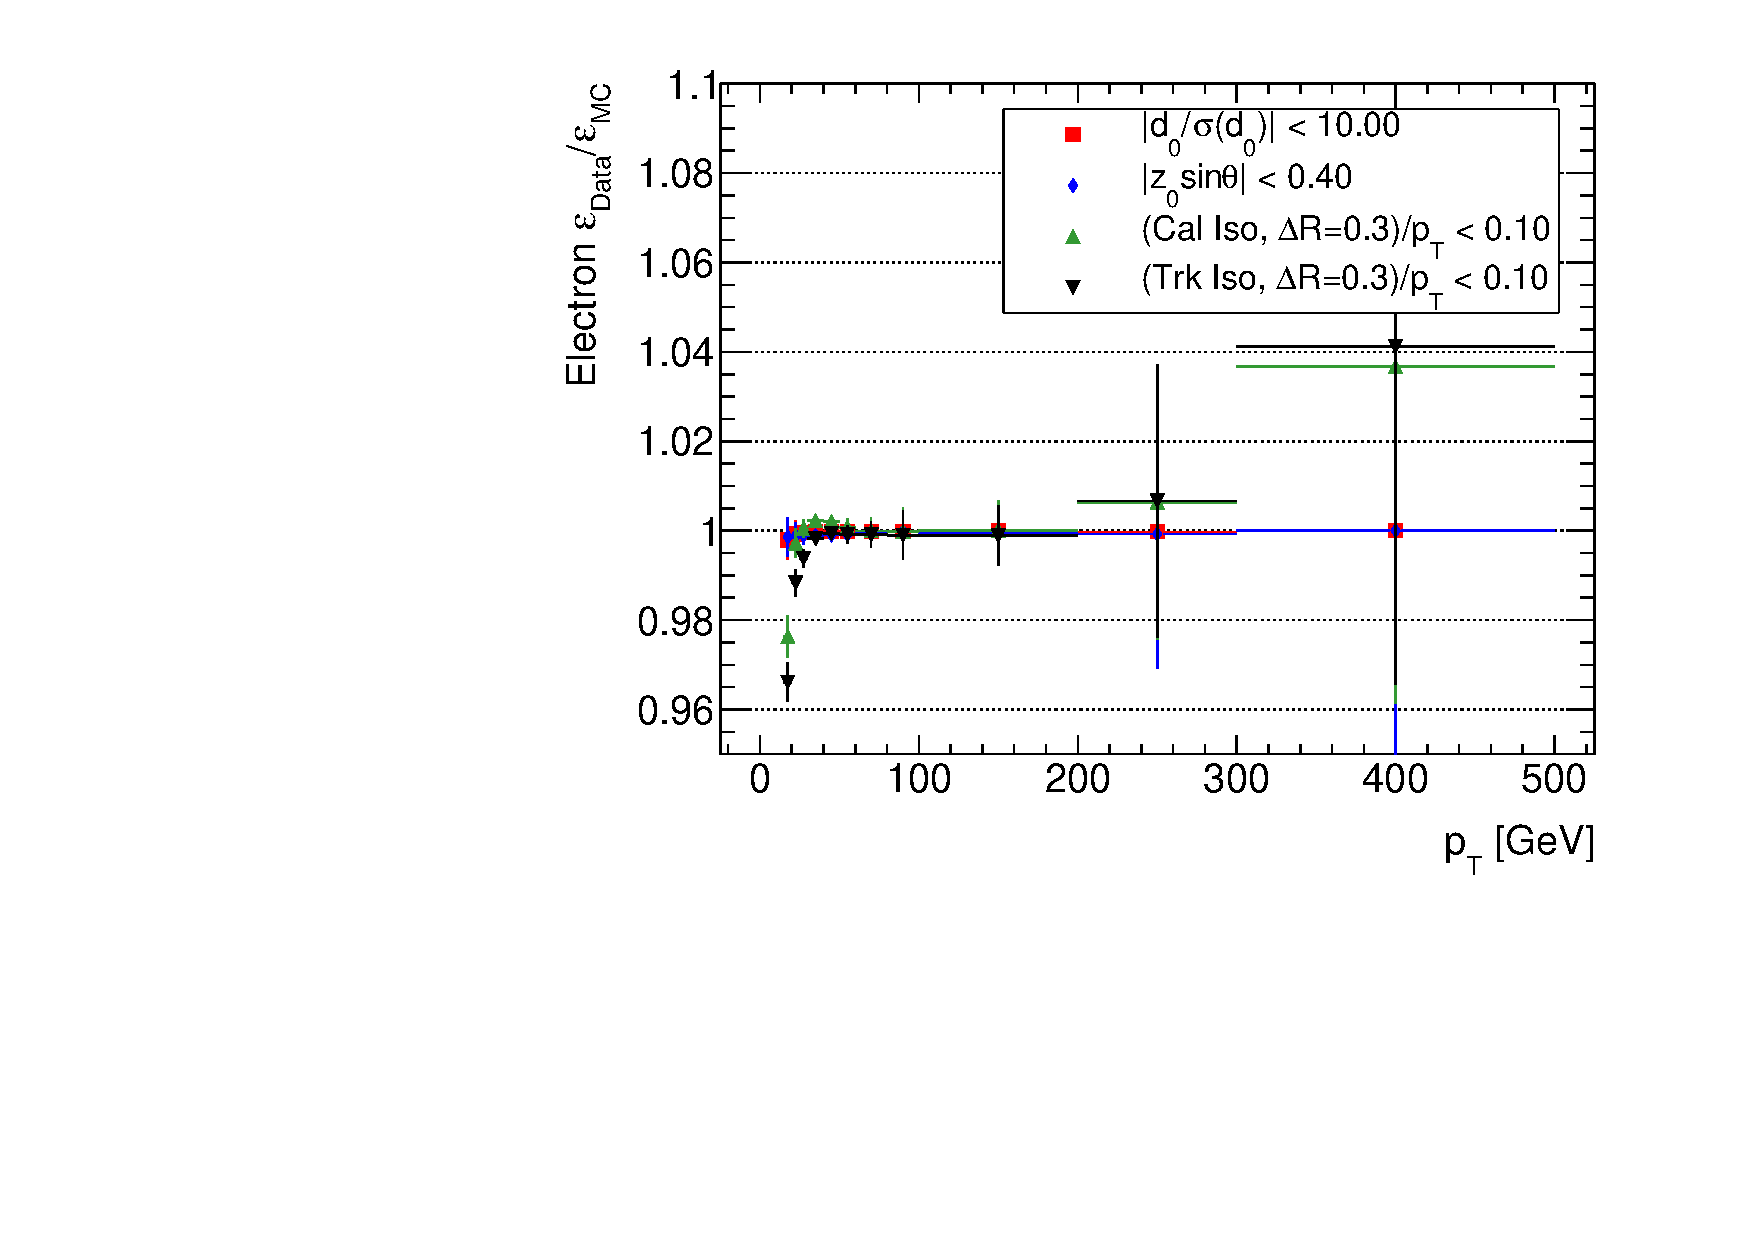
\includegraphics[width=.48\columnwidth]{figures/modelindependent/c_e_pt_allSF}
  }
  \hfill
  \subfloat[Electron $|\eta|$ Scale Factors]{
    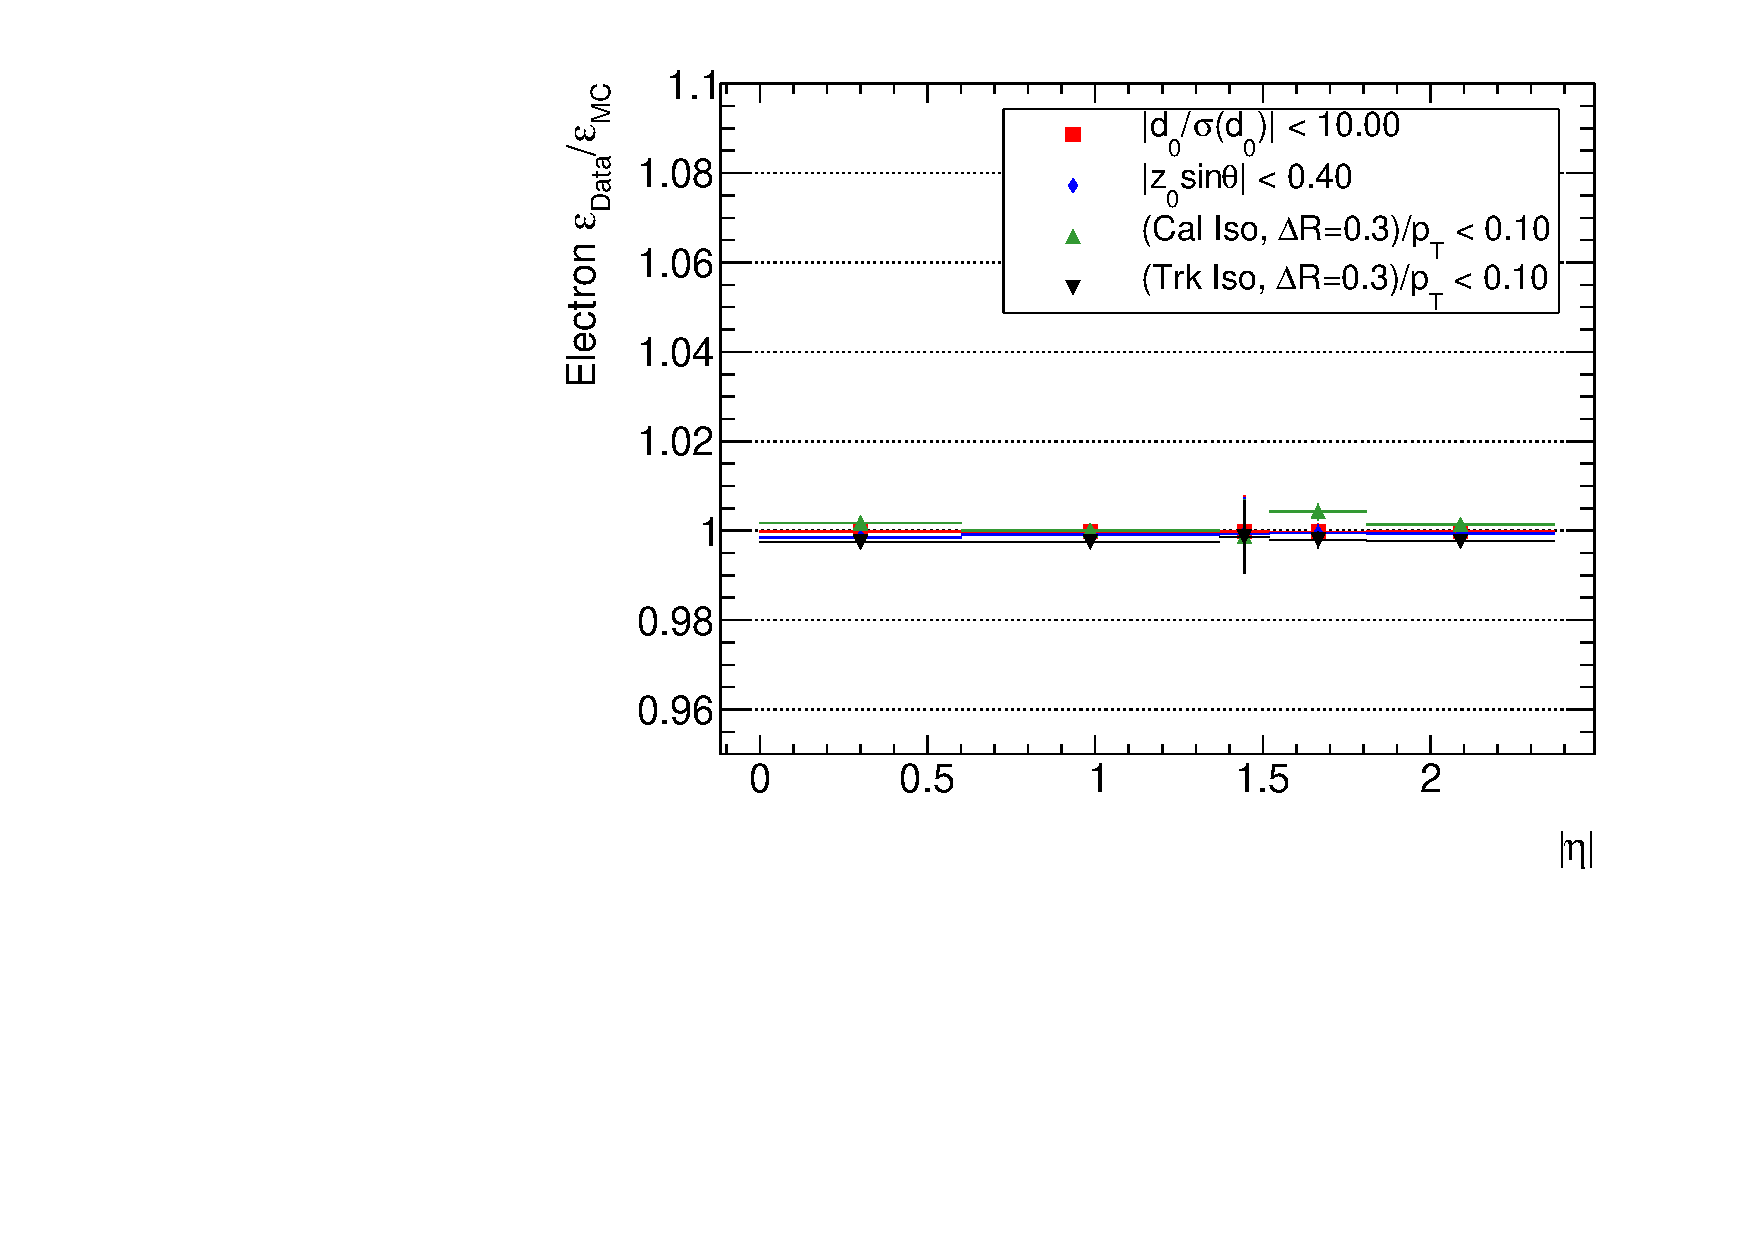
\includegraphics[width=.48\columnwidth]{figures/modelindependent/c_e_eta_allSF}
  } \\
  \subfloat[Muon \pt\ Scale Factors]{
    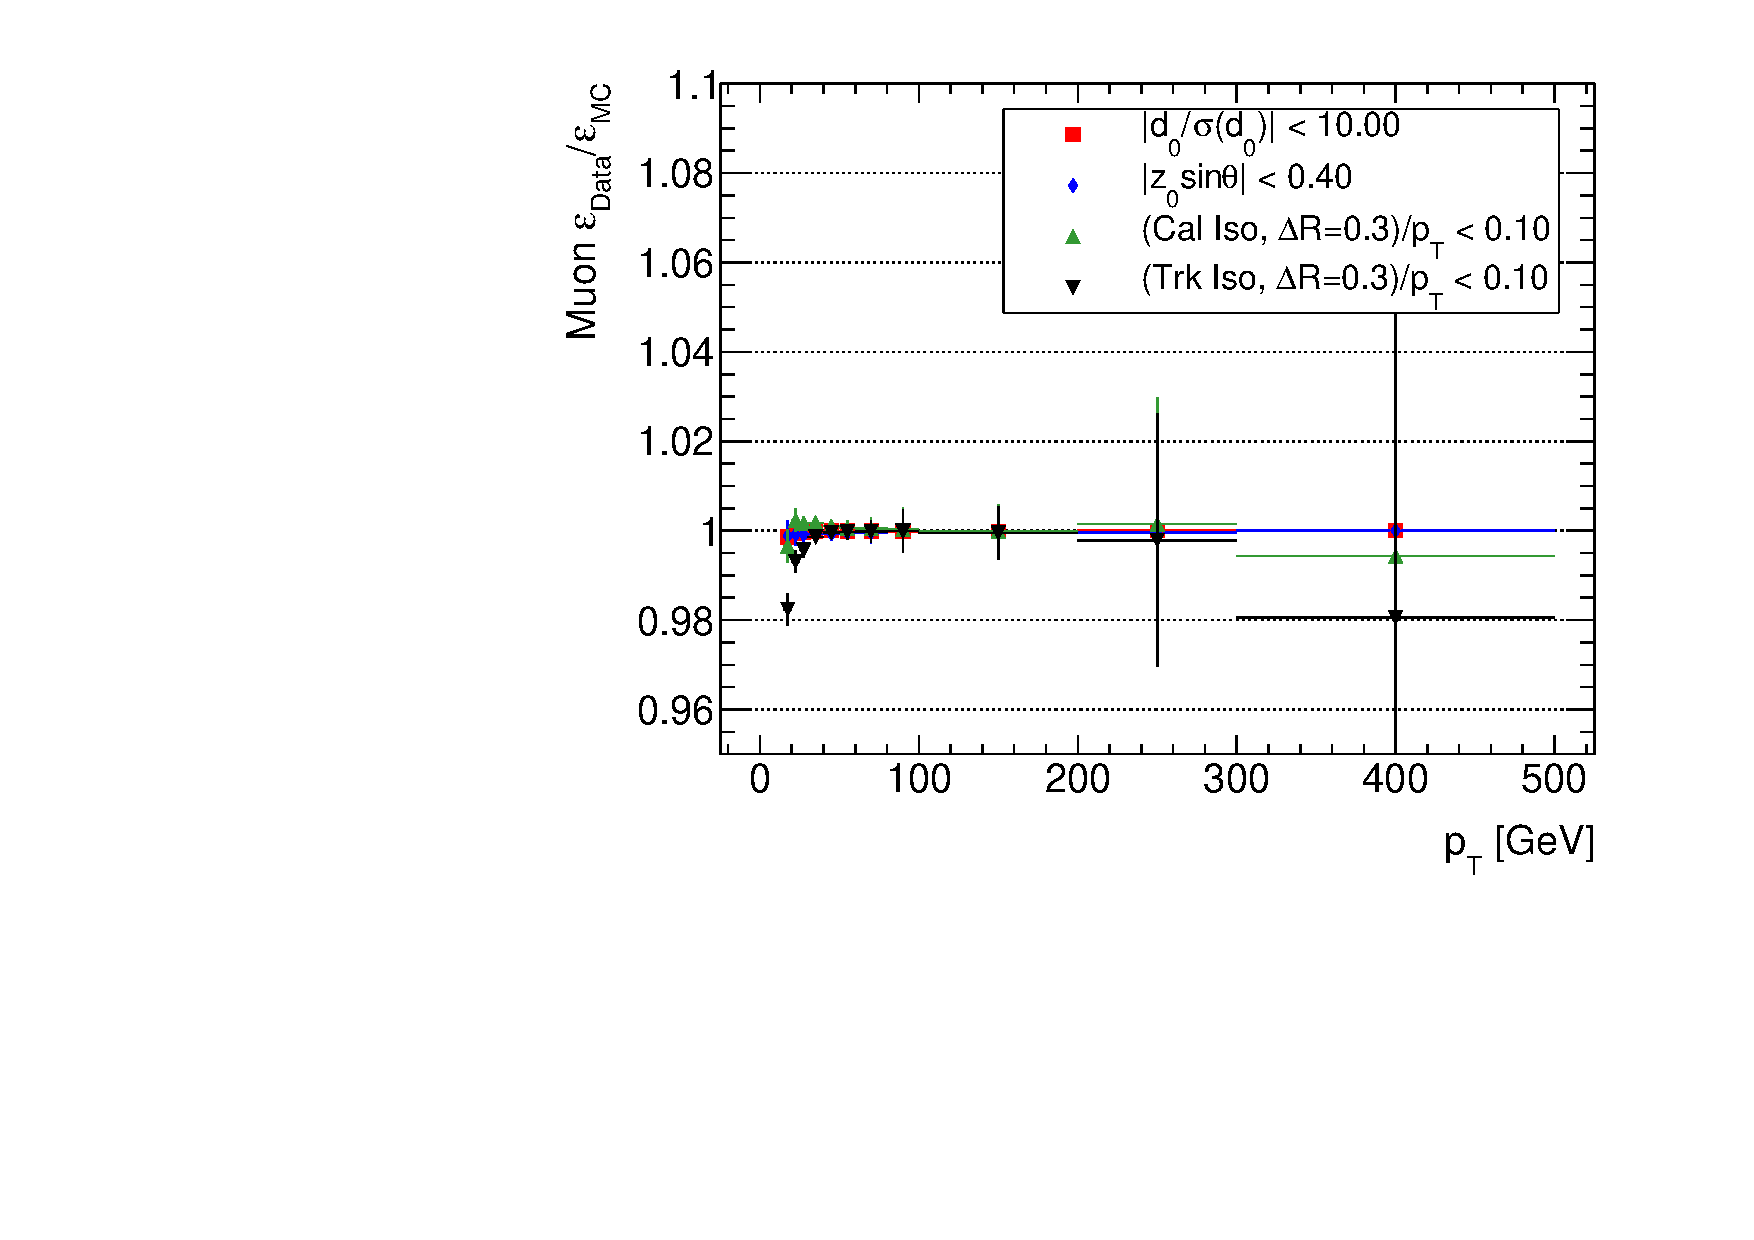
\includegraphics[width=.48\columnwidth]{figures/modelindependent/c_m_pt_allSF}
  }
  \hfill
  \subfloat[Muon $|\eta|$ Scale Factors]{
    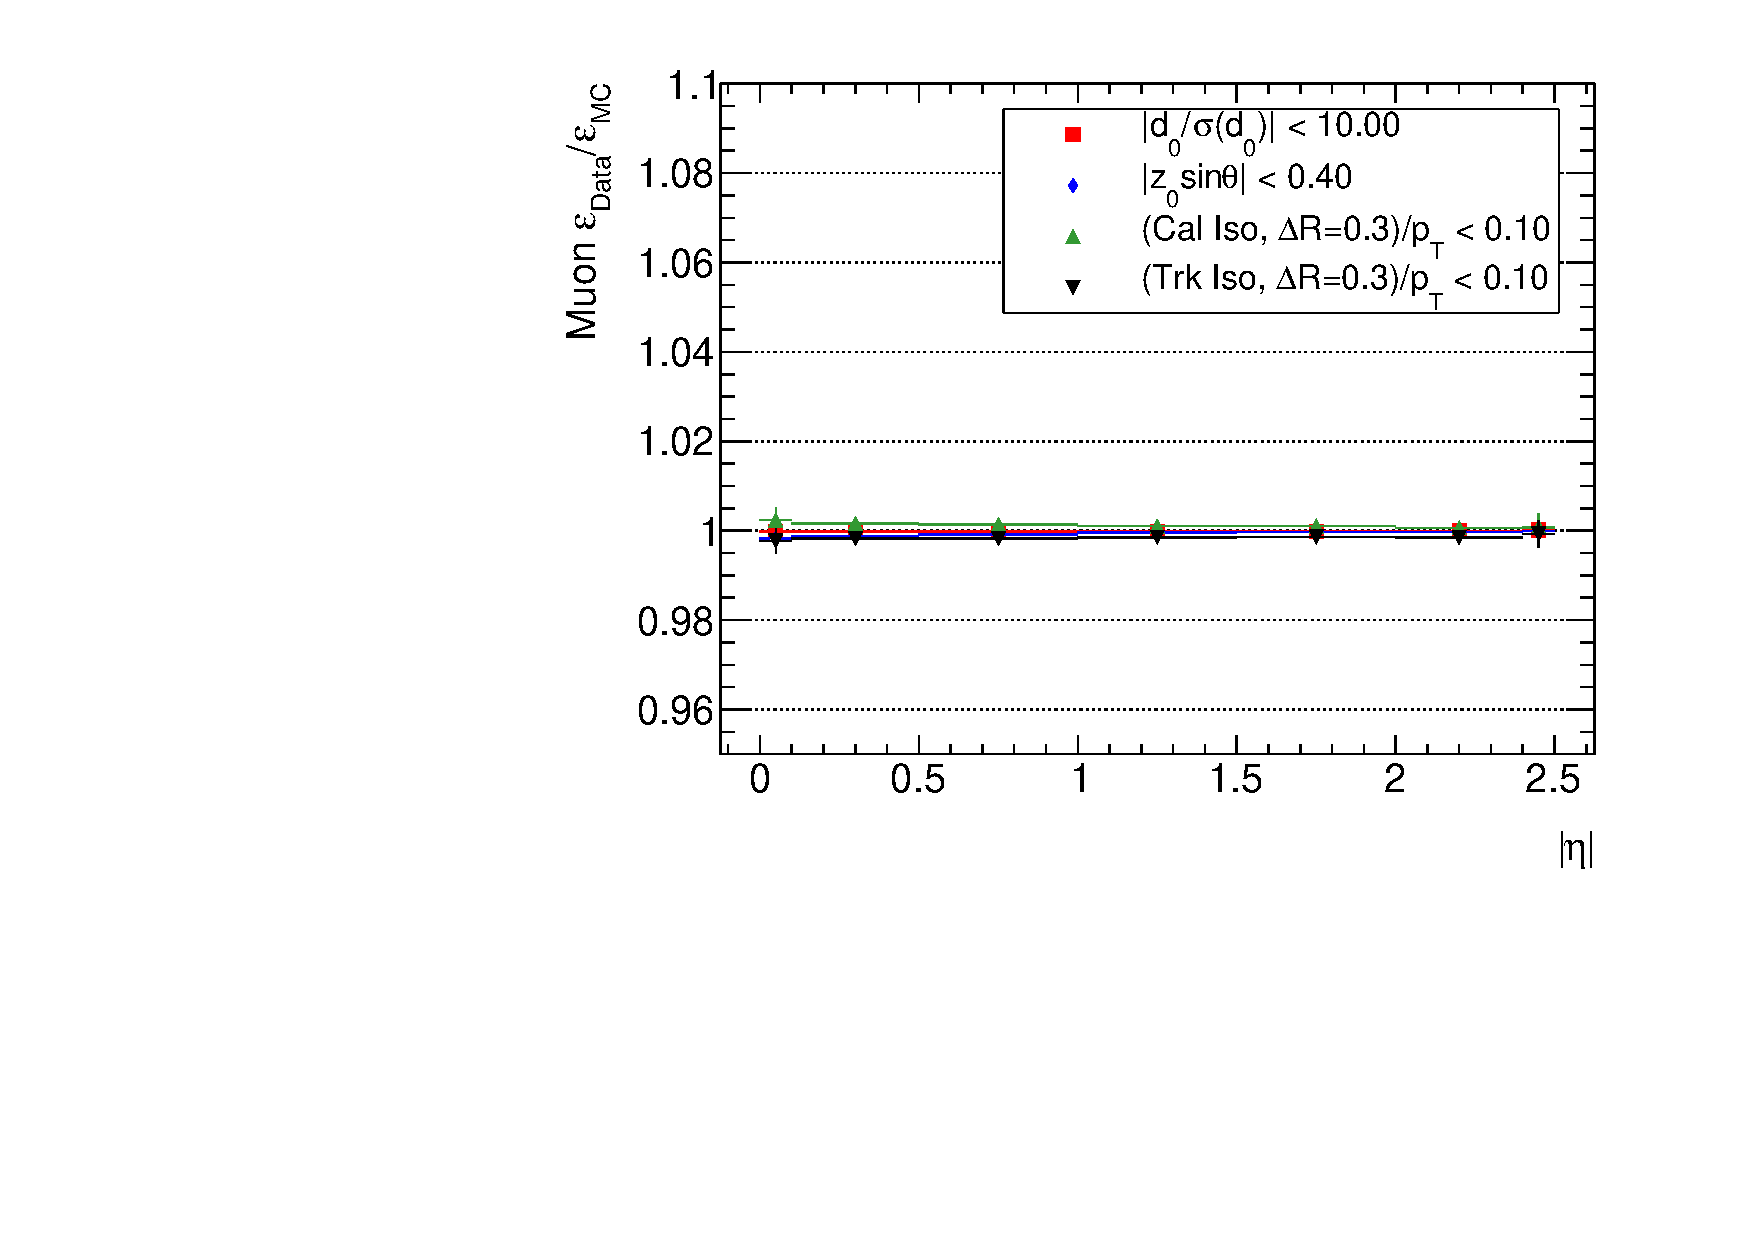
\includegraphics[width=.48\columnwidth]{figures/modelindependent/c_m_eta_allSF}
  }
  \caption{Scale factors for electrons and muons as functions of \pt\ (left) and $|\eta|$ (right).}
  \label{fig:model-independent-lepton-SFs}
\end{figure}

The $\mu\tau_{\mathrm{had}}$ region applies addition cuts to reduce the large contribution from fake tau leptons in $W$+jets events:

\begin{itemize}
	\item $\cos{\Delta\phi(\mu, \met)} + \cos{\Delta\phi(\tau, \met)} >$ -0.15,
	\item $\Delta\phi(\mu, \tau_{had}) >$ 2.4,
	\item $m_{\mathrm{T}}^{\mu} < 50 \GeV$,
	\item $42< m_{Z}^{vis.} < 82 \GeV$, and
	\item $\pt^{\mu} < 40 \GeV$.
\end{itemize}

The $\pt$ and $\eta$ distributions of the $\mu$ and $\tau_{\mathrm{had}}$ are shown in figure~\ref{fig:model-independent-VR-mutau}.

\begin{figure}[htbp]
	\subfloat[Leading Lepton \pt]
		{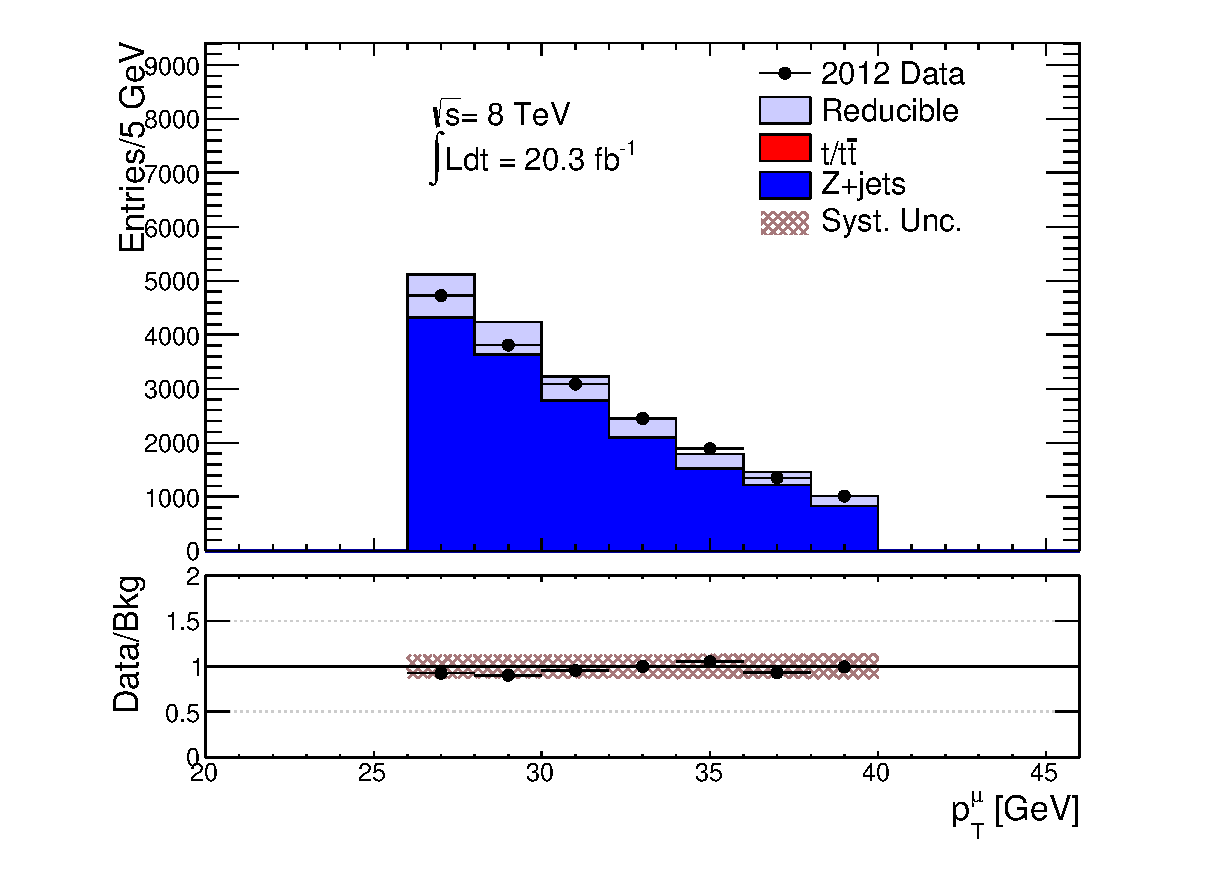
\includegraphics[width=.48\columnwidth]{figures/modelindependent/OSZ_LeadingPt.eps}}
  \hfill
	\subfloat[Leading Lepton $|\eta|$]
		{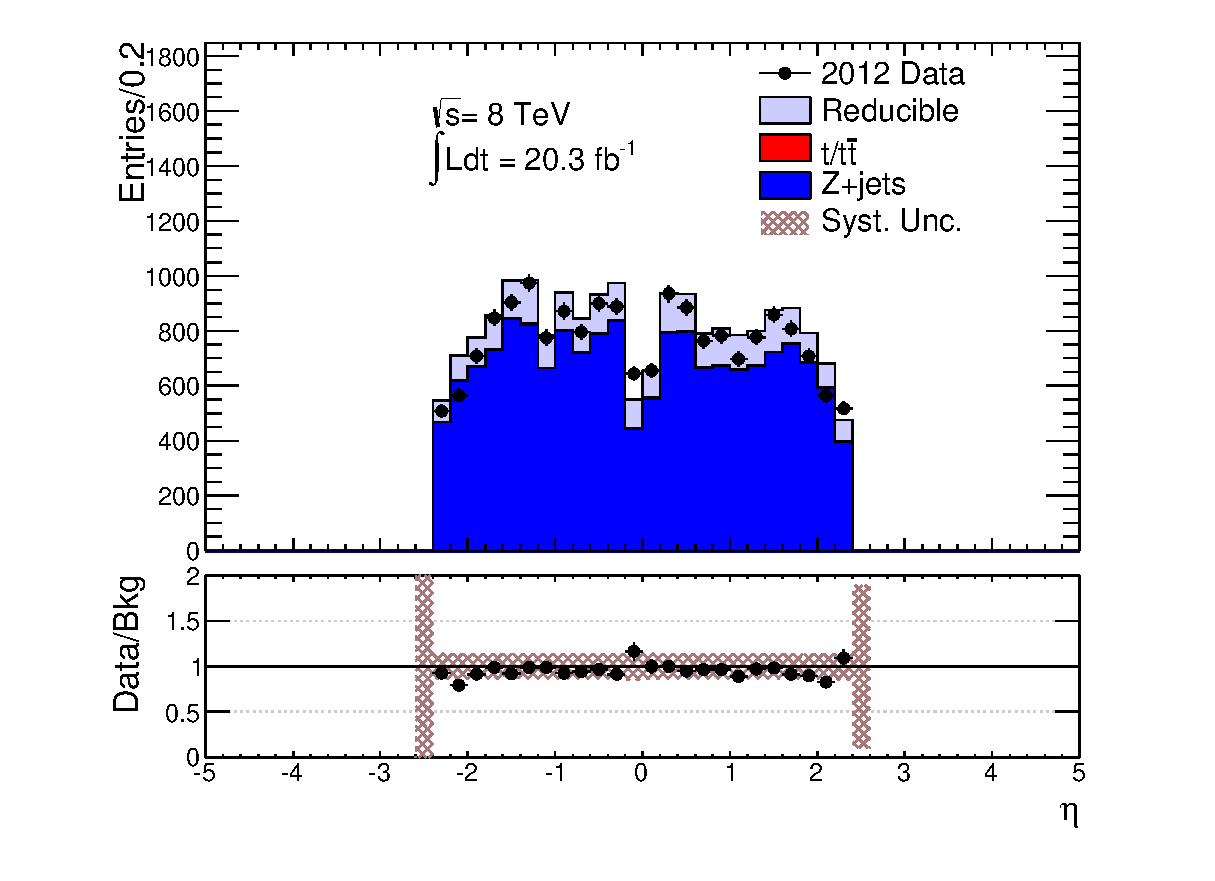
\includegraphics[width=.48\columnwidth]{figures/modelindependent/OSZ_LeadingEta.eps}} \\
	\subfloat[Subleading Lepton \pt]
		{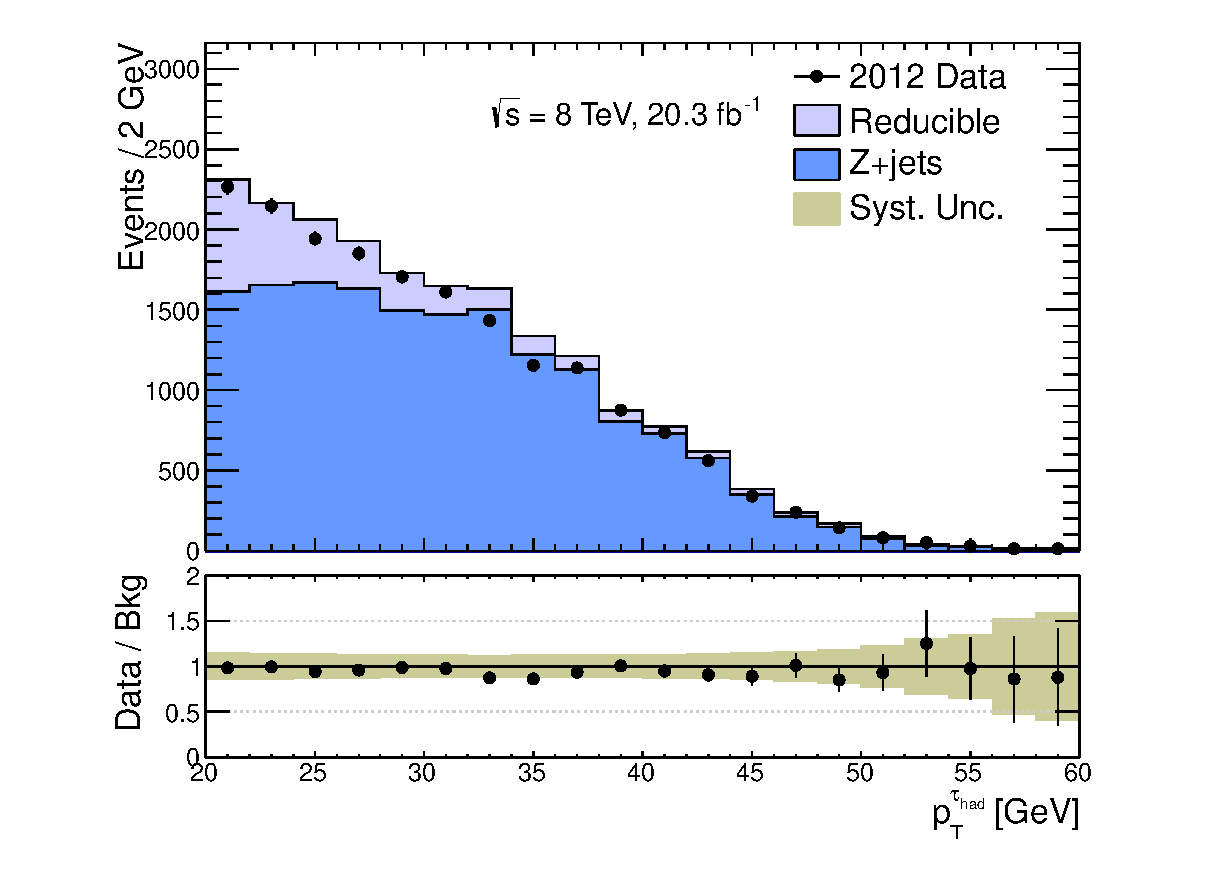
\includegraphics[width=.48\columnwidth]{figures/modelindependent/OSZ_SubleadPt.eps}}
  \hfill
	\subfloat[Subleading Lepton $|\eta|$]
		{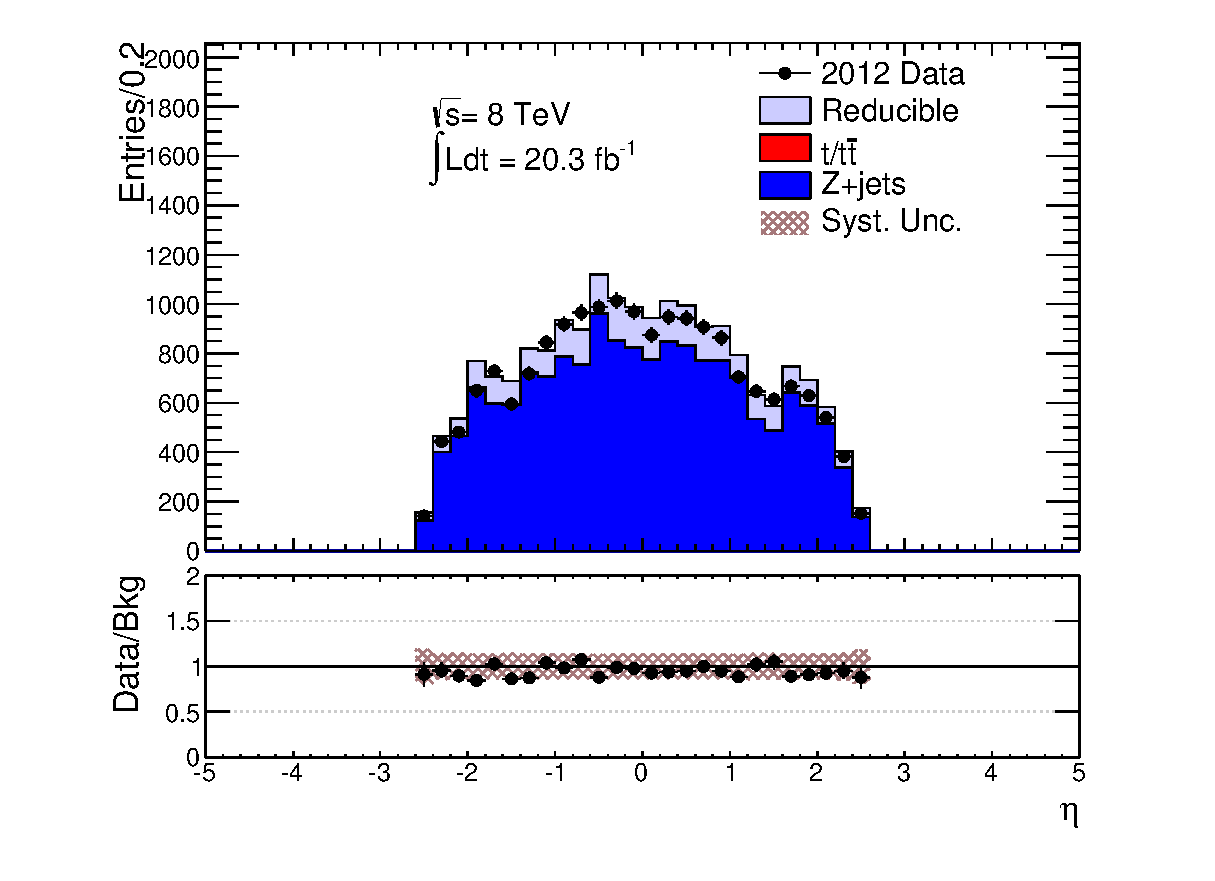
\includegraphics[width=.48\columnwidth]{figures/modelindependent/OSZ_SubleadEta.eps}}
	\caption{$\pt$ and $\eta$ distribution of the muon and the hadronically decaying tau lepton in the $\mu\tau_{\mathrm{had}}$ validation region.}
	\label{fig:model-independent-VR-mutau}
\end{figure}


\subsection{$t\overline{t}$ Validation Regions}\label{sec:model-independent-validation-regions-ttbar}
In signal regions that veto $Z$ bosons and require large $\Htjets$ or $\Etmiss$, a large reducible background component is expected from $t\overline{t}$ events, where both $W$ bosons decay leptonically and a third lepton arises from a misidentified jet or semileptonic heavy flavor decay. This process is tested in the $t\overline{t}$ validation regions, which require at least one $b$-tagged jet with $\pt>30 \GeV$, exactly two electrons or muons with the same charge, and $\Ht<500 \GeV$. The requirement that the leptons have the same sign vetoes dilepton $t\overline{t}$ events with two prompt leptons from $W$ decays, while the $\Ht$ requirement reduces the potential contamination from new BSM phenomena. Note that events containing hadronically decaying tau leptons are used to derive a systematic uncertainty on the tau fake factors due to the flavor composition of the events (section~\ref{sec:ff-tau-systematics}), and so are not used as a validation region. 

The $\pt$ and $\eta$ distributions of the leading and subleading leptons are shown in figure~\ref{fig:model-independent-VR-ttbar}.

\begin{figure}[tbp]
  \subfloat[Leading Lepton \pt]{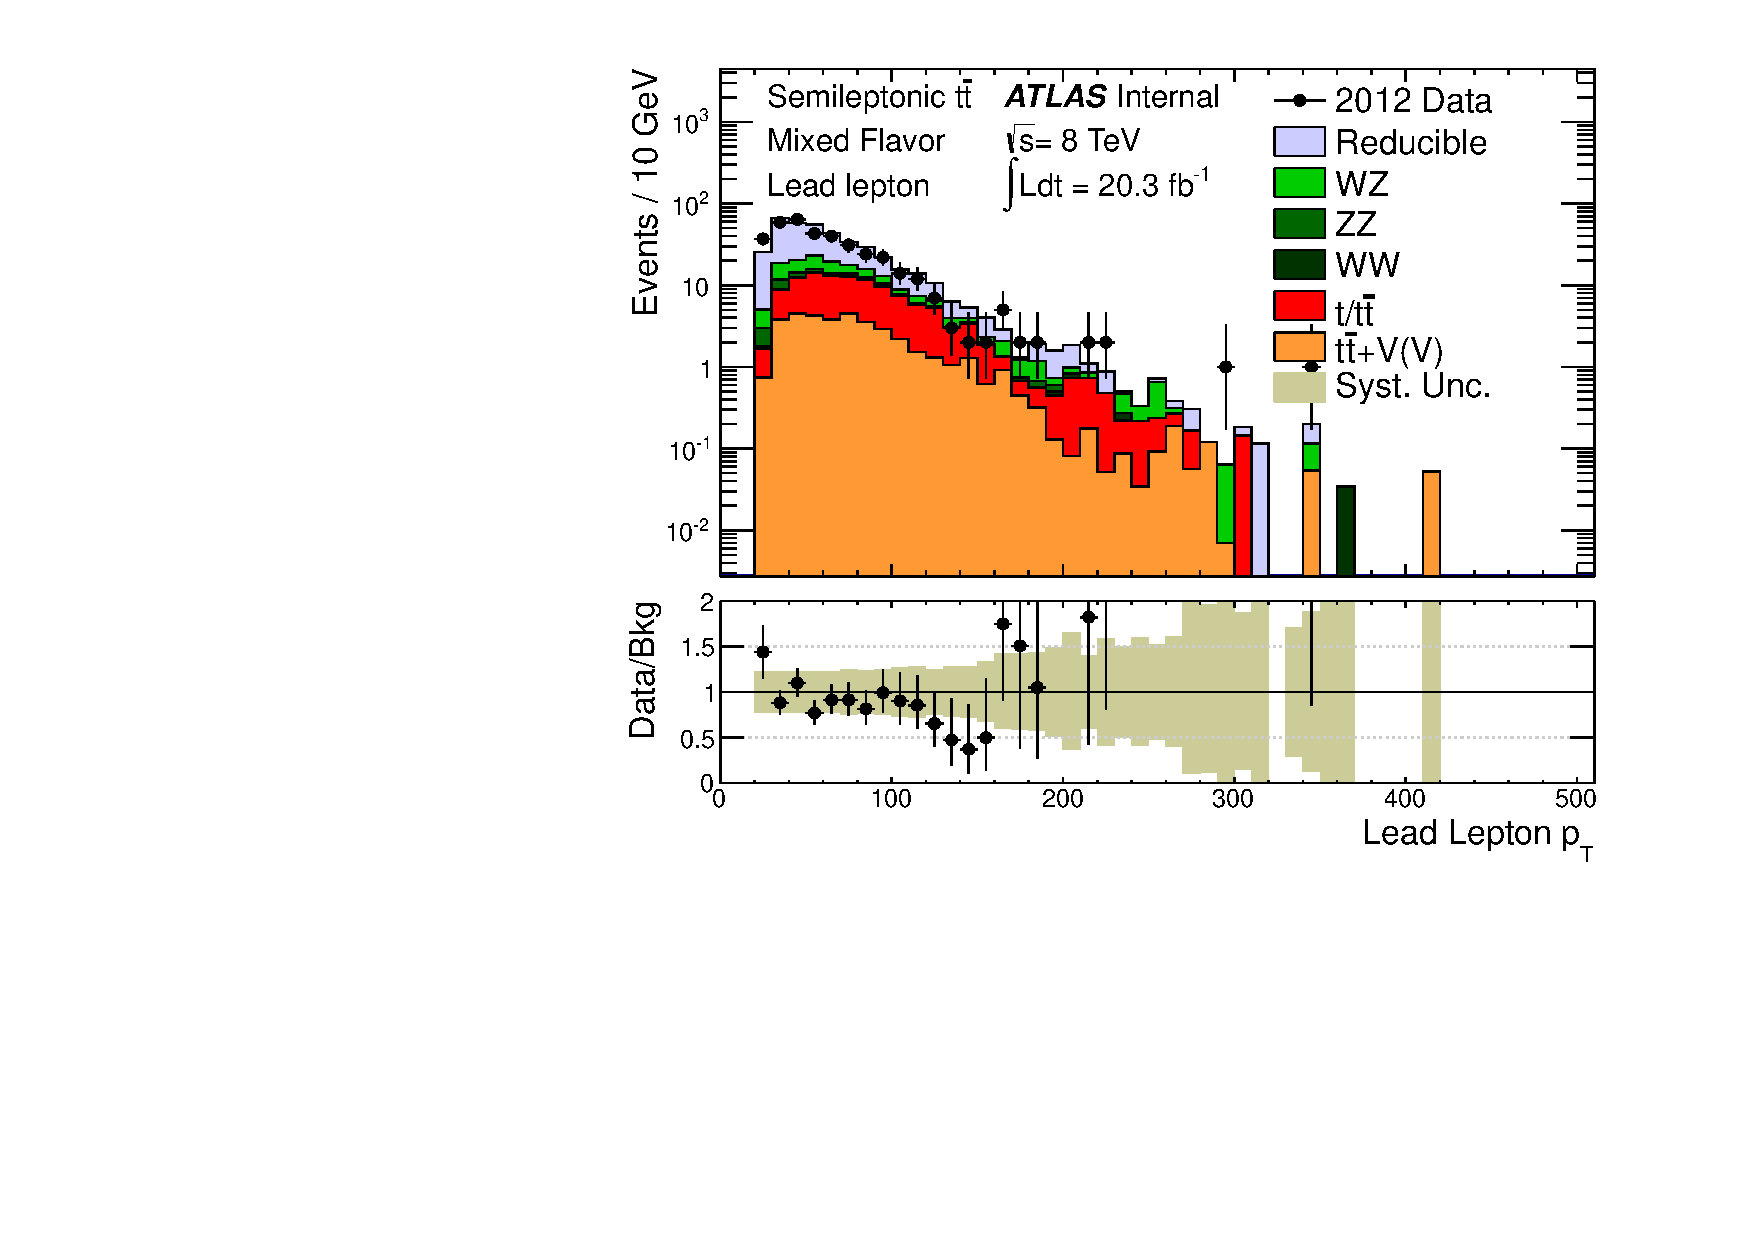
\includegraphics[width=.48\columnwidth]{figures/modelindependent/semileptop_emu_mue_LeadPt}}
  \hfill
  \subfloat[Leading Lepton $|\eta|$]{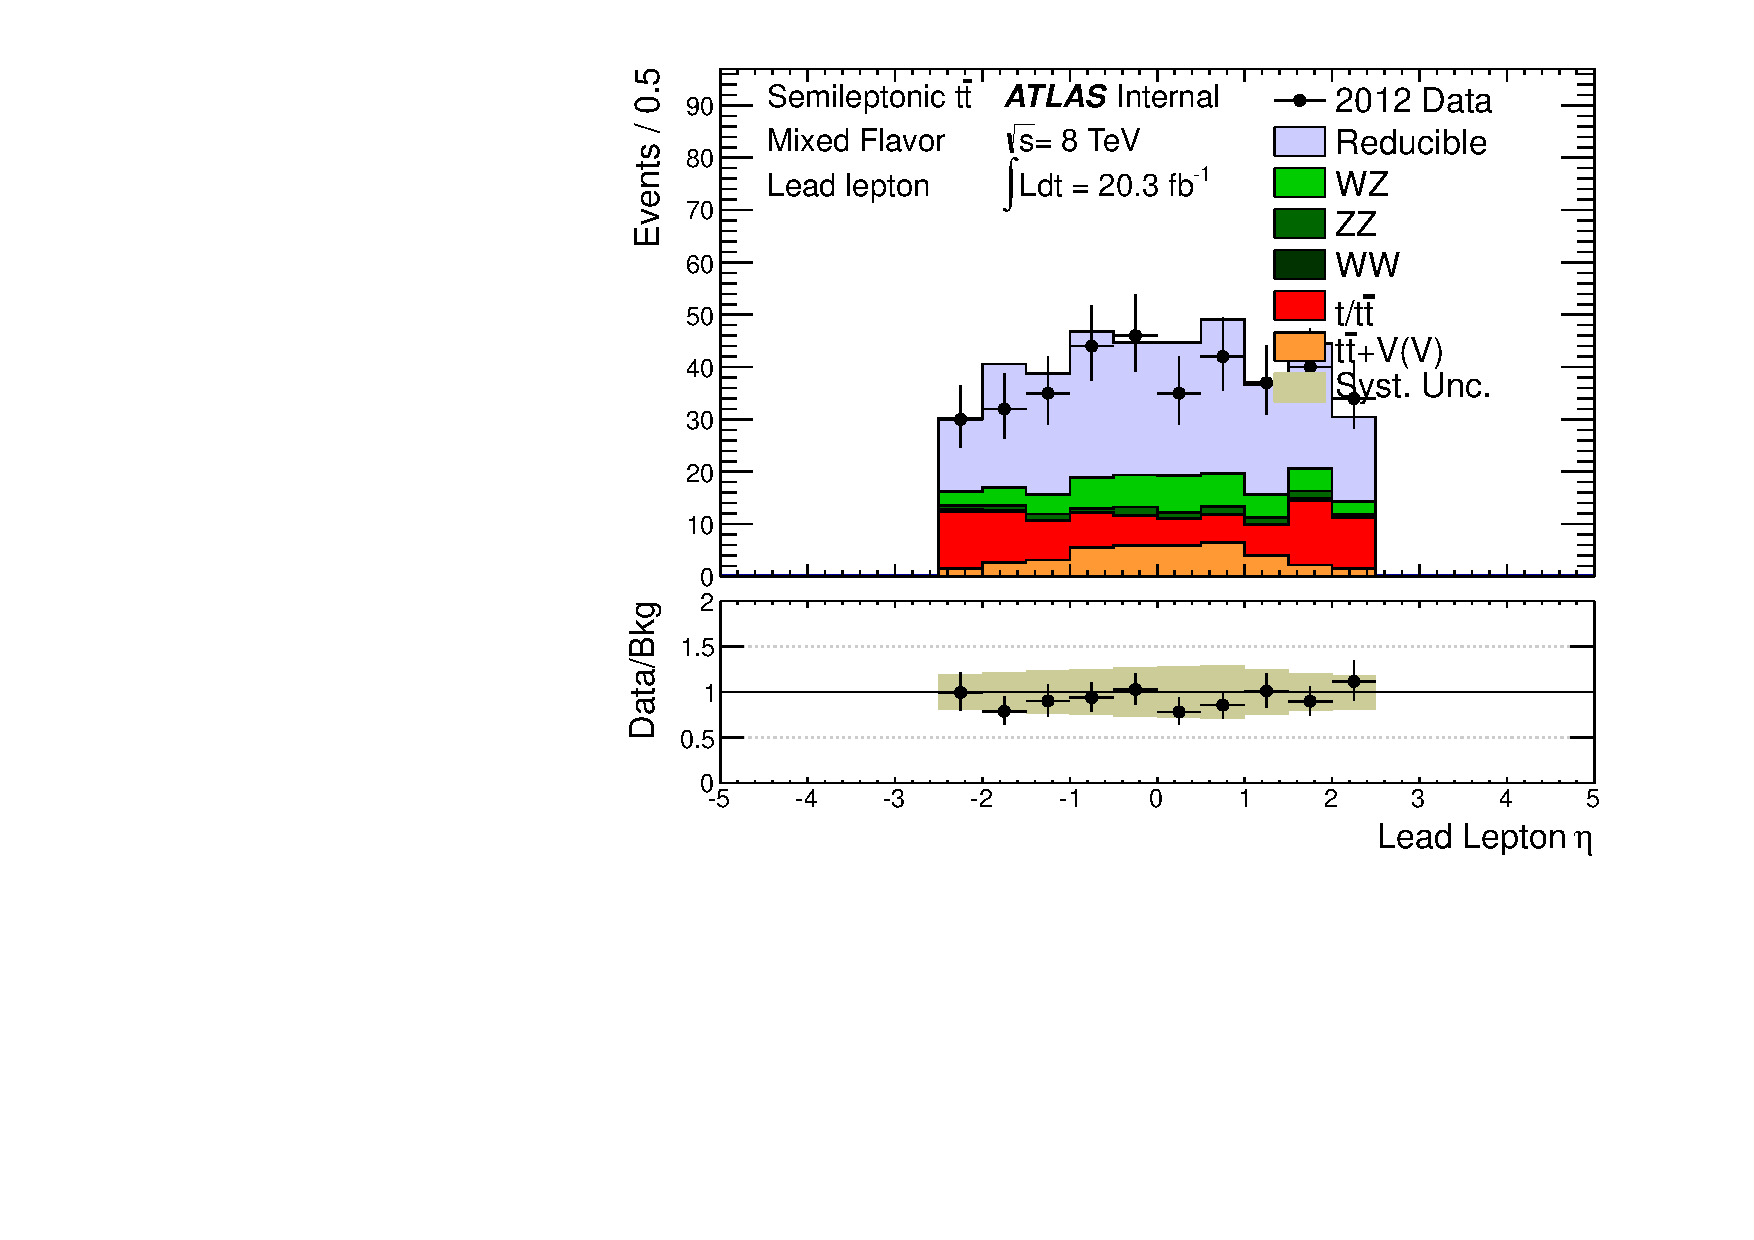
\includegraphics[width=.48\columnwidth]{figures/modelindependent/semileptop_emu_mue_LeadEta}} \\
  \subfloat[Subleading Lepton \pt]{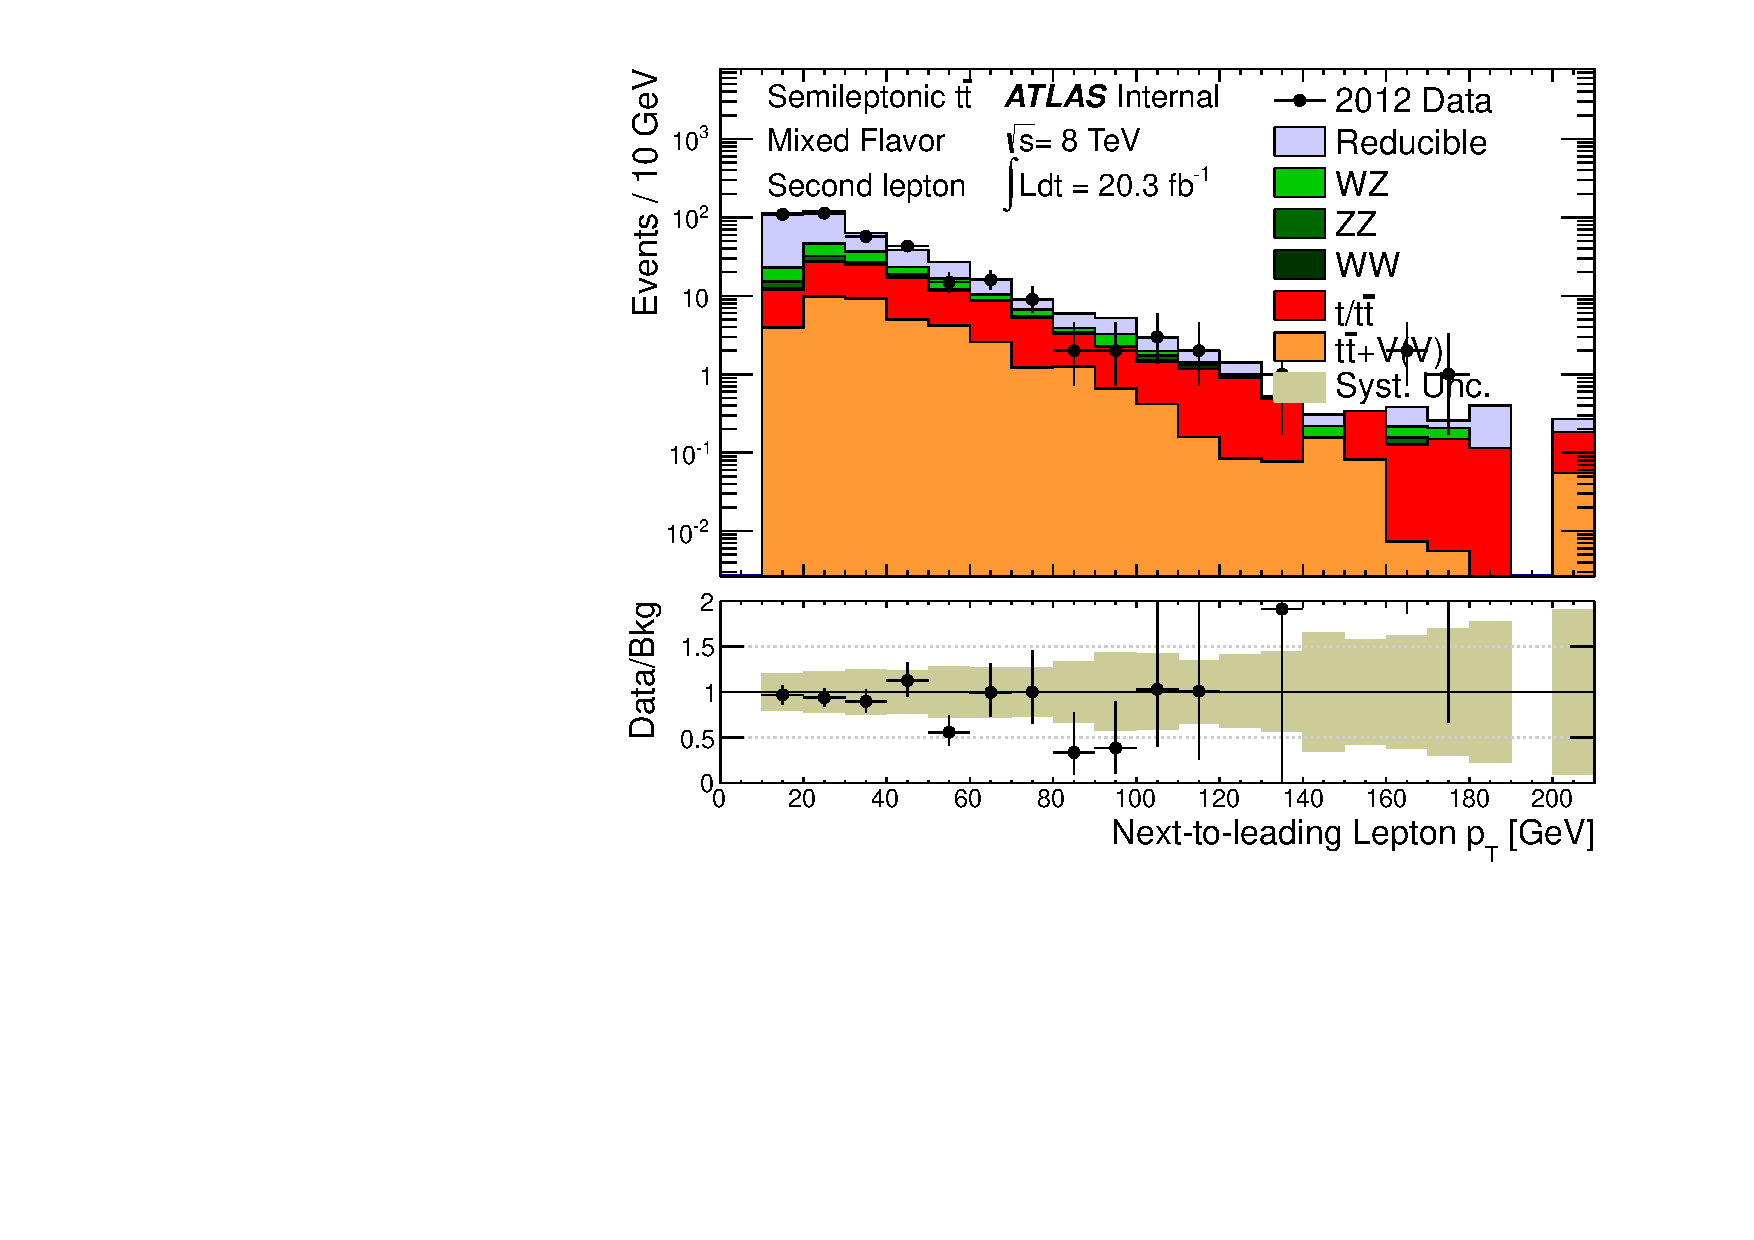
\includegraphics[width=.48\columnwidth]{figures/modelindependent/semileptop_emu_mue_SubleadPt}}
  \hfill
  \subfloat[Subleading Lepton $|\eta|$]{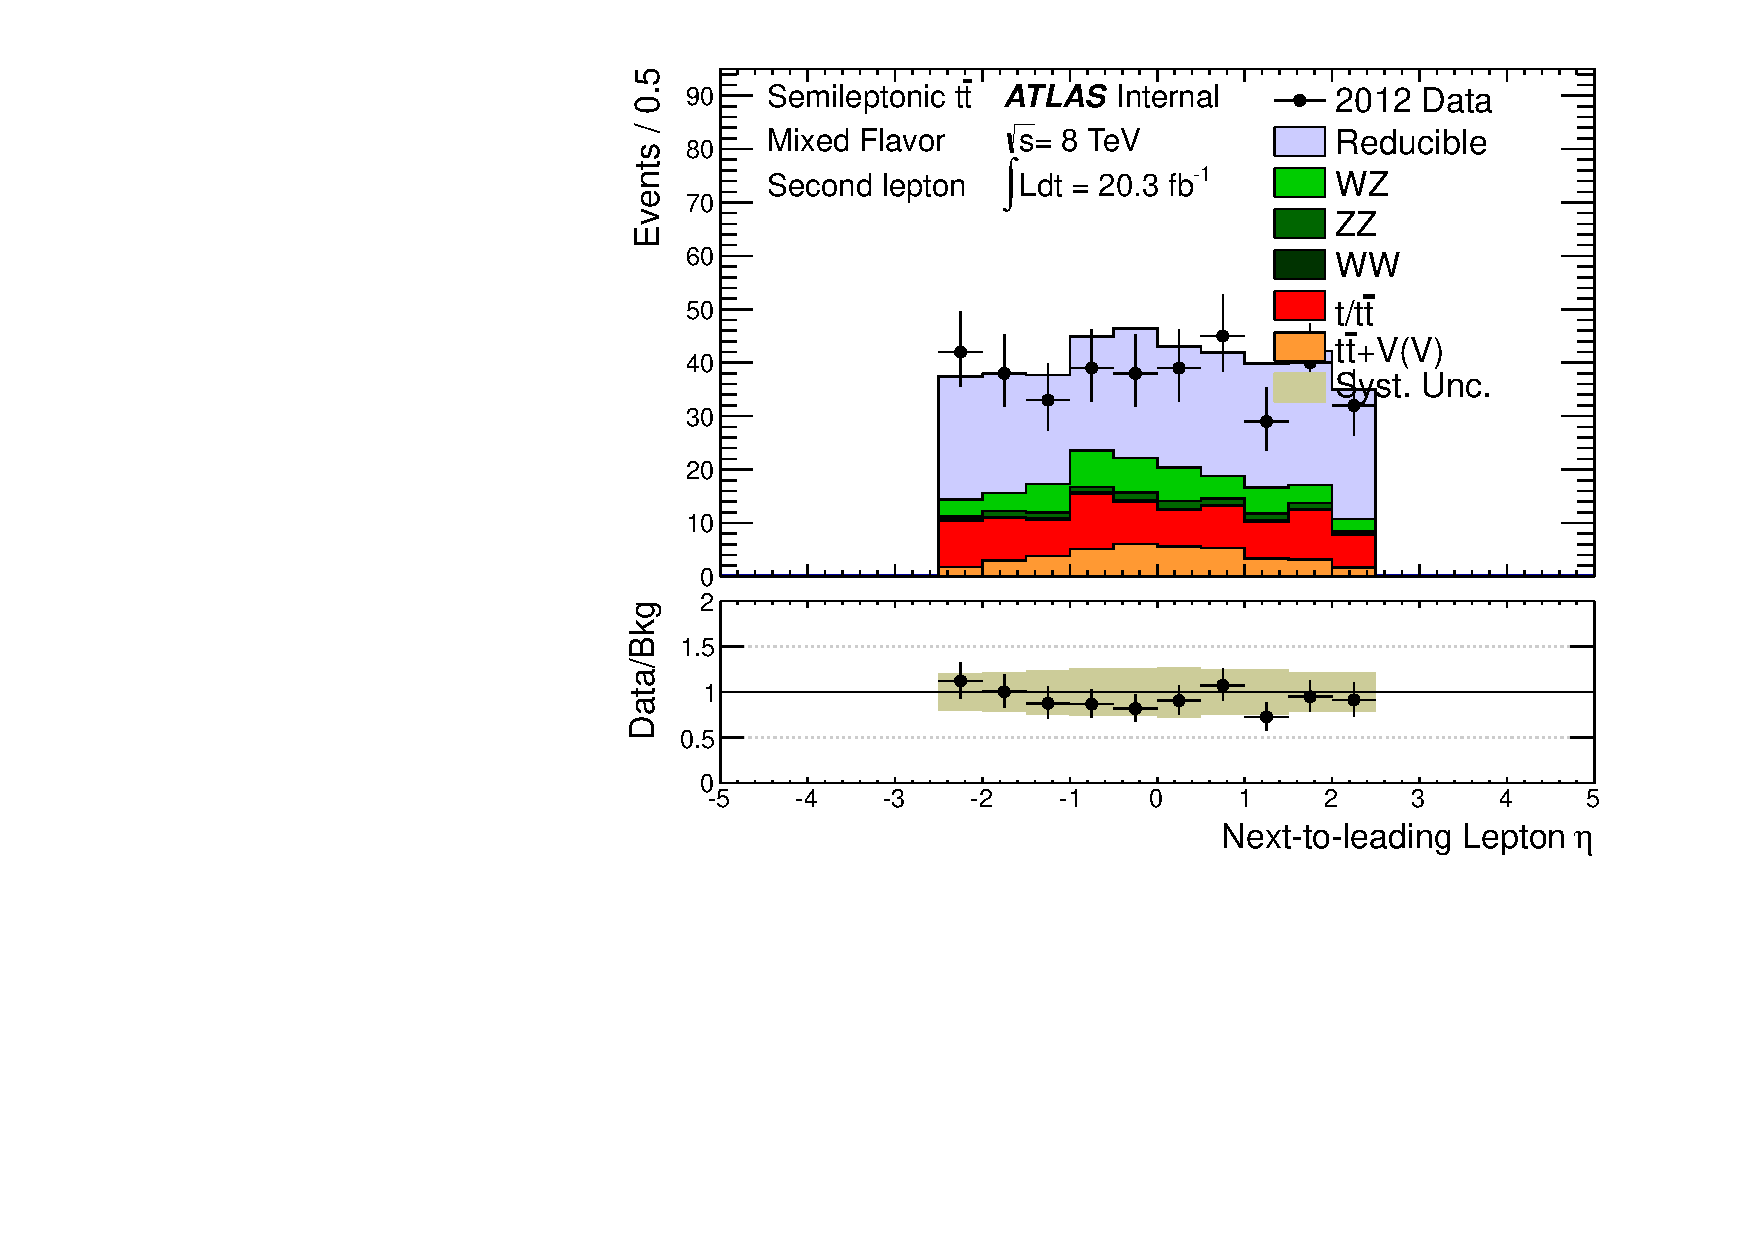
\includegraphics[width=.48\columnwidth]{figures/modelindependent/semileptop_emu_mue_SubleadEta}} \\
  \subfloat[\meff]{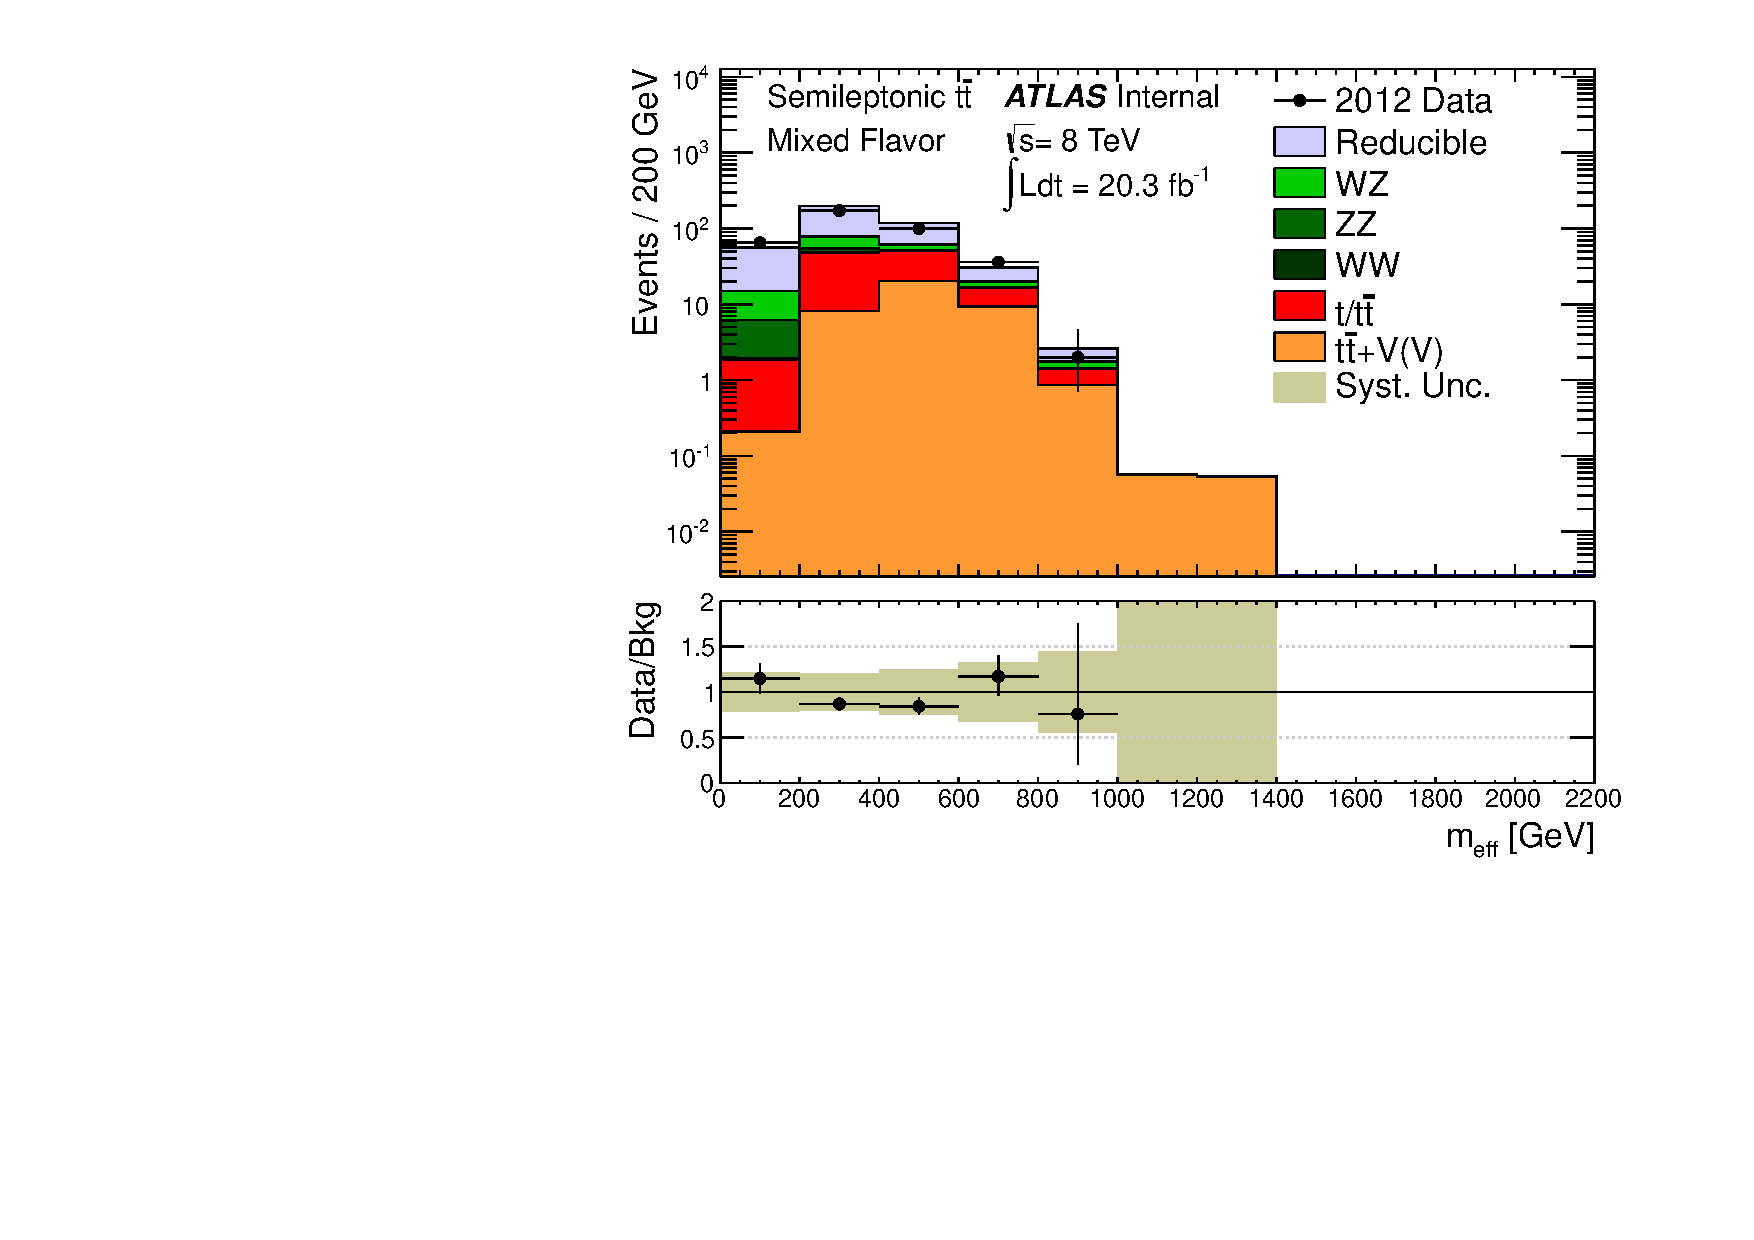
\includegraphics[width=.48\columnwidth]{figures/modelindependent/semileptop_emu_mue_ST}}
  \hfill
  \subfloat[\met]{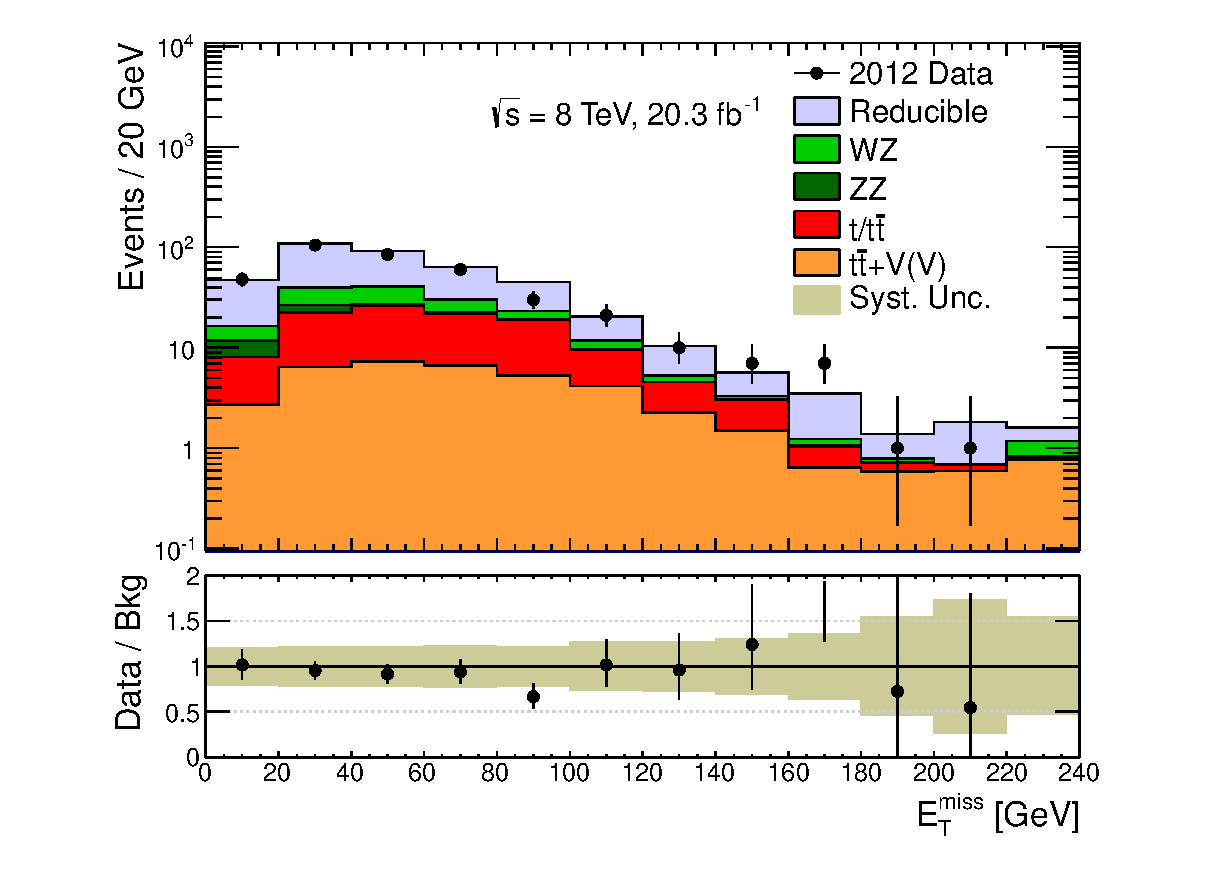
\includegraphics[width=.48\columnwidth]{figures/modelindependent/semileptop_emu_mue_MET}}
  \caption{\ttbar\ validation regions for all flavor ($e, \mu$) combinations.}
  \label{fig:model-independent-VR-ttbar}
\end{figure}

\subsection{Intermediate Fake Factor Validation Regions}\label{sec:model-independent-validation-regions-intermediate-ff}
The fake factor method is further validated in regions containing events with two signal (numerator) leptons and one ``intermediate'' lepton, which fulfills selection criteria looser than the numerator criteria but tighter than the denominator criteria. Separate fake factors are derived for intermediate leptons; these are defined schematically as $\langle$intermediate$\rangle/\langle$denominator$\rangle$, rather than $\langle$numerator$\rangle/\langle$denominator$\rangle$. Specifically, the intermediate leptons satisfy most of the numerator criteria except for:

\begin{itemize}
	\item \textbf{Electrons}: the electron must pass the \texttt{medium++} cuts, but fail the \texttt{tight++} cuts.  
	\item \textbf{Muons}: the candidate must have either its track or calorimeter transverse isolation energy
	satisfy $0.10 < \mathrm{iso}/\pt < 0.15$.
	\item \textbf{Taus}: the tau candidate must pass the \texttt{Medium-BDT} identification requirement, but fail the
	\texttt{tight-BDT} identification requirement.
\end{itemize}

The first two regions, targeting reducible electrons and muons, require an OSSF pair of electrons or muons, plus a third intermediate electron or muon of different flavor. The events are largely due to $Z\rightarrow ee$ or $Z\rightarrow \mu\mu$ events, with an additional lepton that is either prompt and fails the signal lepton criteria, or is due to a reducible process. 

\begin{figure}[tbp]\centering
  \subfloat[Event Composition]{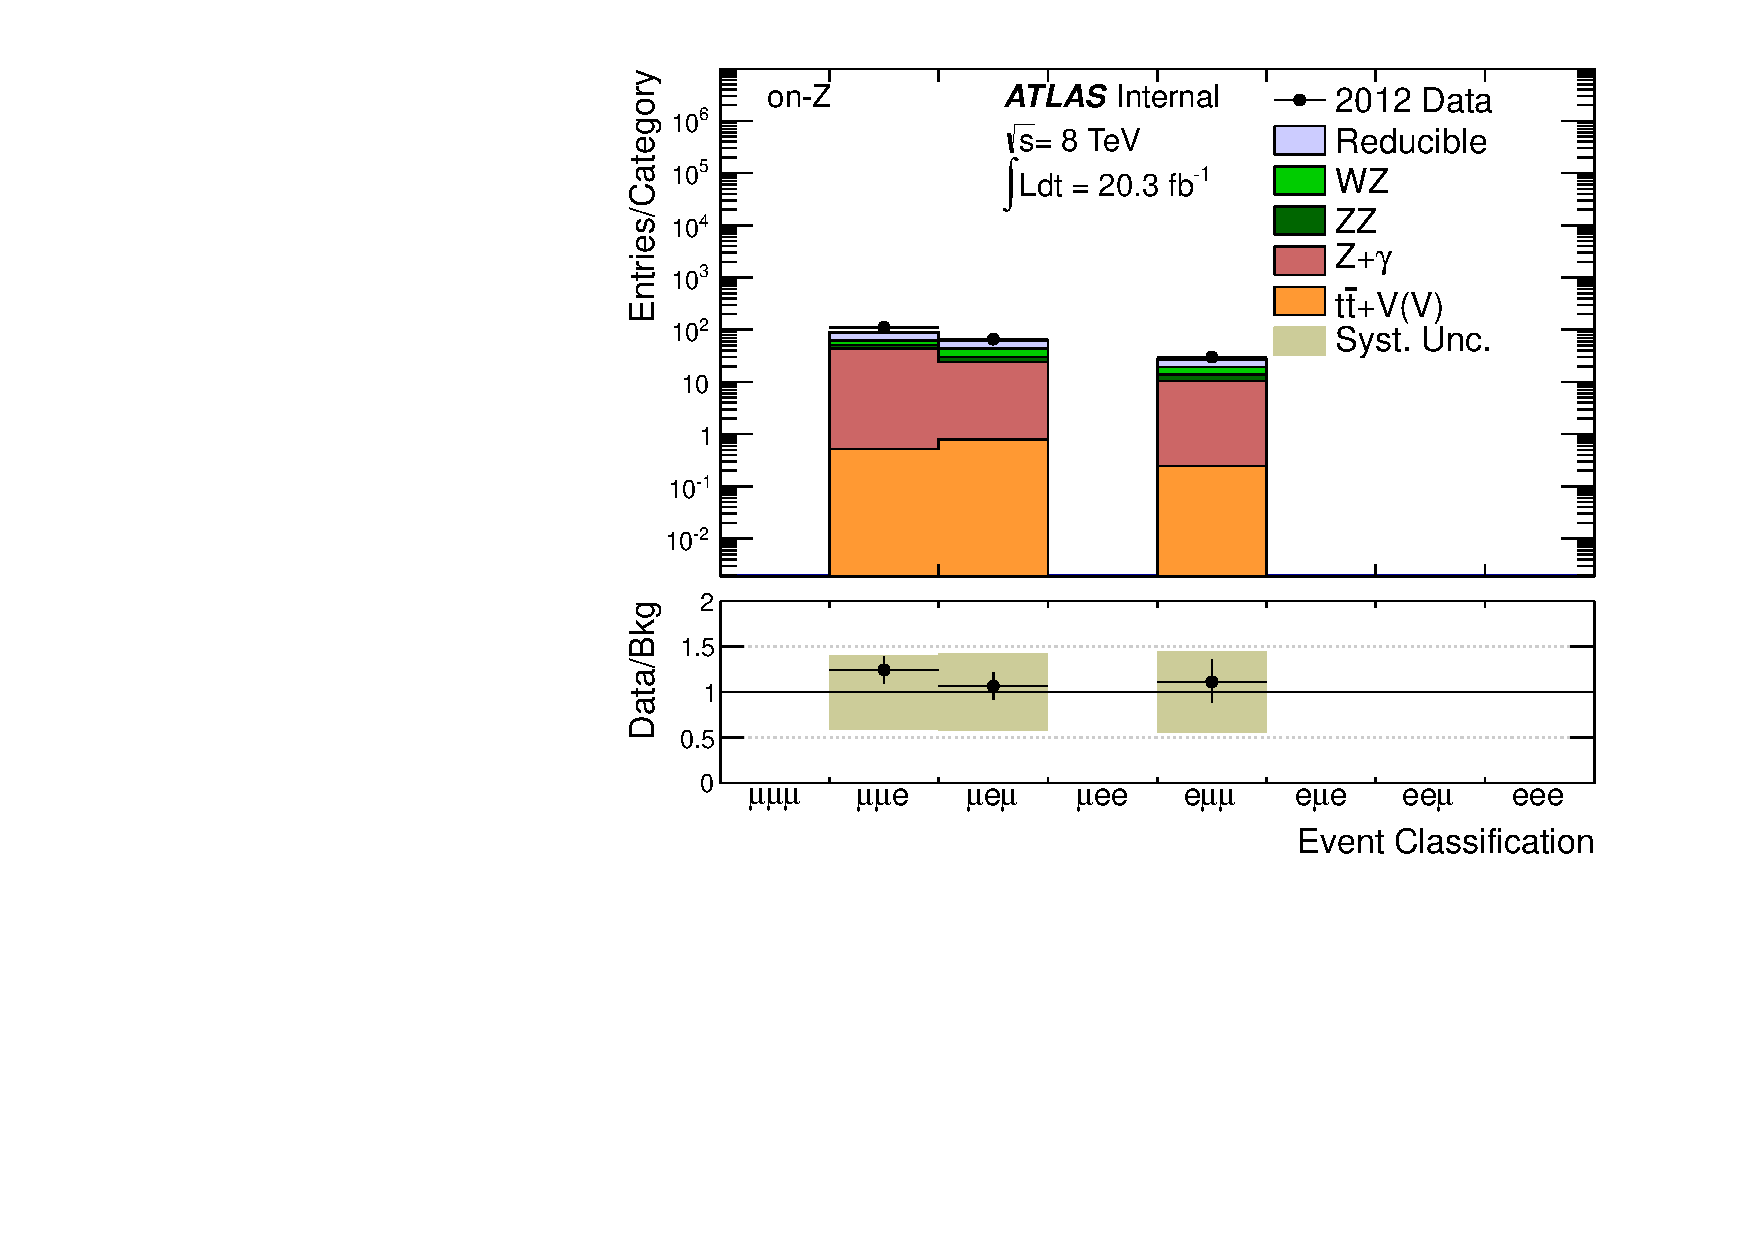
\includegraphics[width=.48\columnwidth]{figures/modelindependent/Z_emu_Zmm_offZe_intelec_Simple3LEventClassification}}
  \hfill
  \subfloat[Electron \pt]{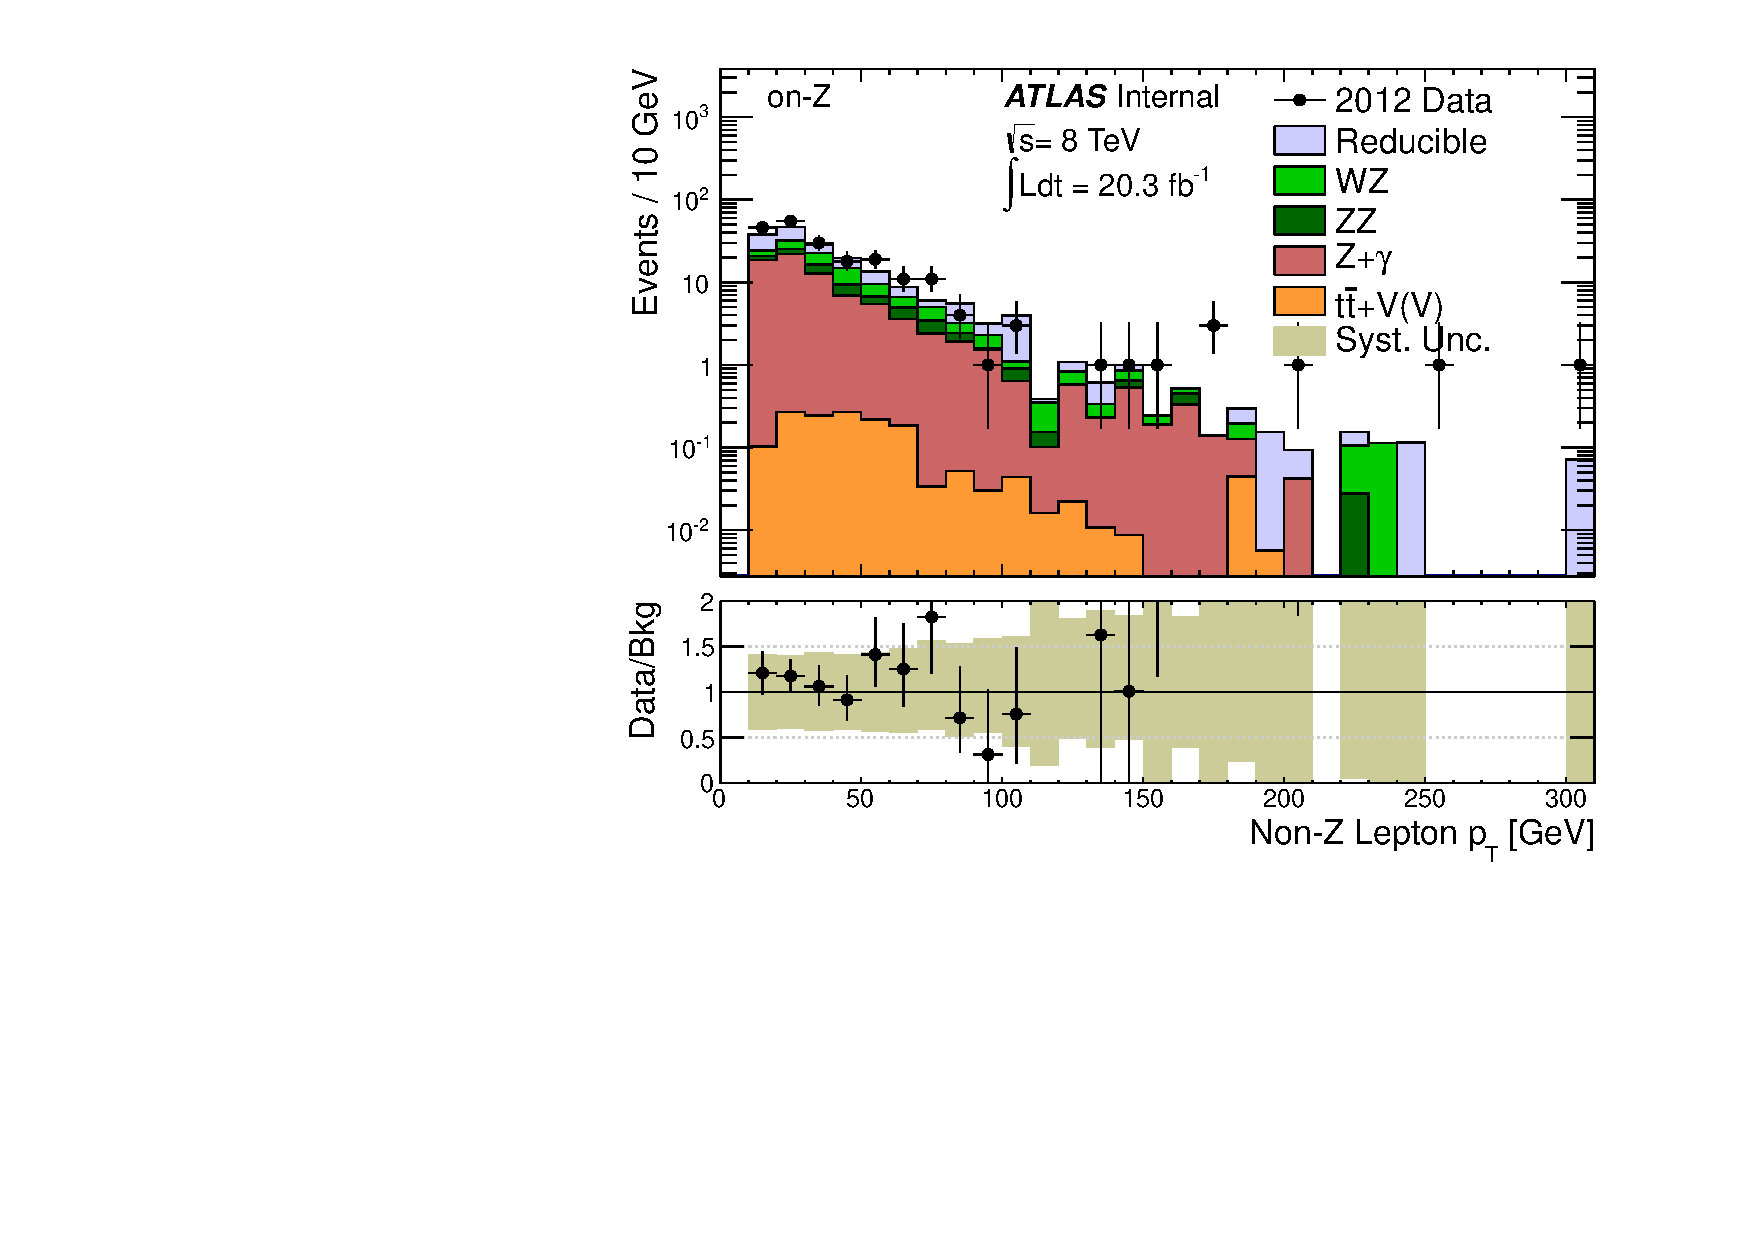
\includegraphics[width=.48\columnwidth]{figures/modelindependent/Z_emu_Zmm_offZe_intelec_OffZPt}} \\
  \subfloat[Electron $\eta$]{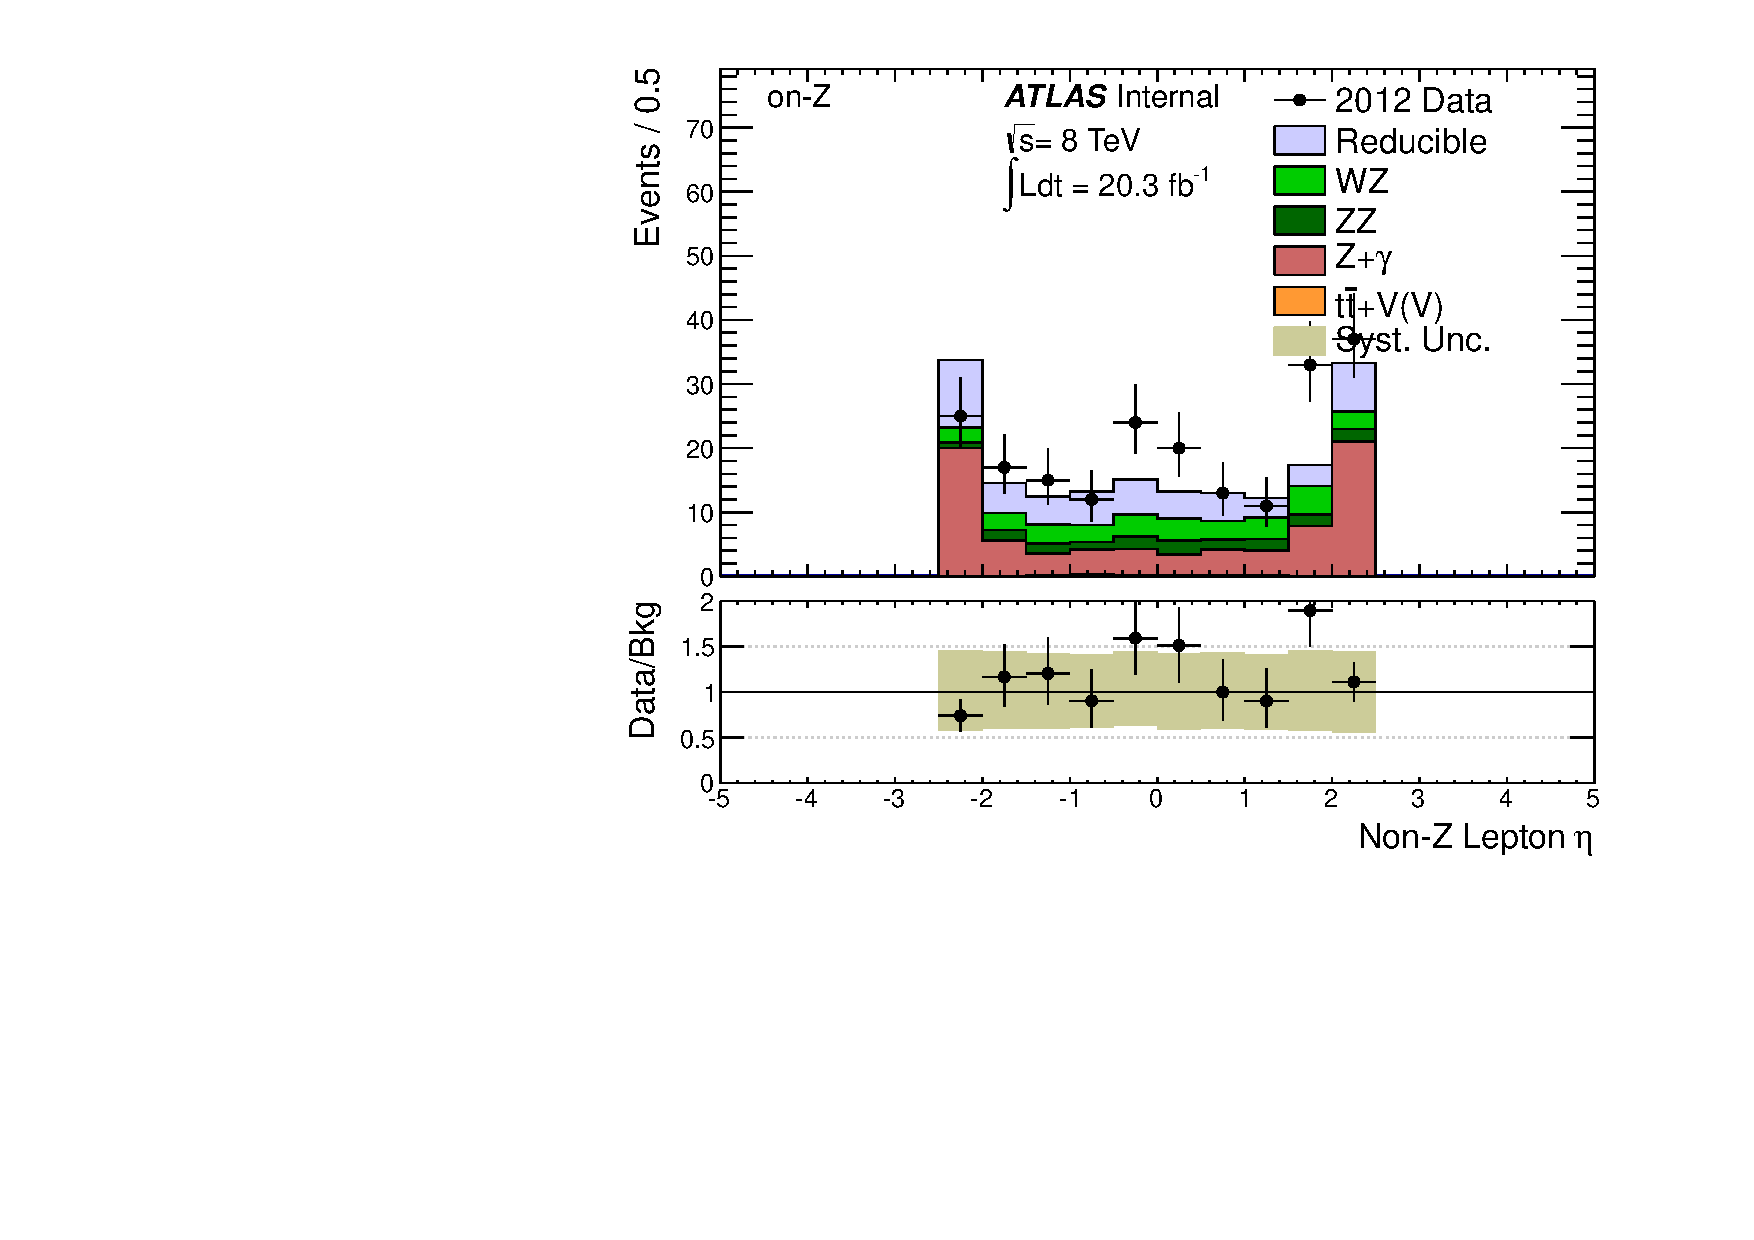
\includegraphics[width=.48\columnwidth]{figures/modelindependent/Z_emu_Zmm_offZe_intelec_OffZEta}}
  \hfill
  \subfloat[Electron \mt]{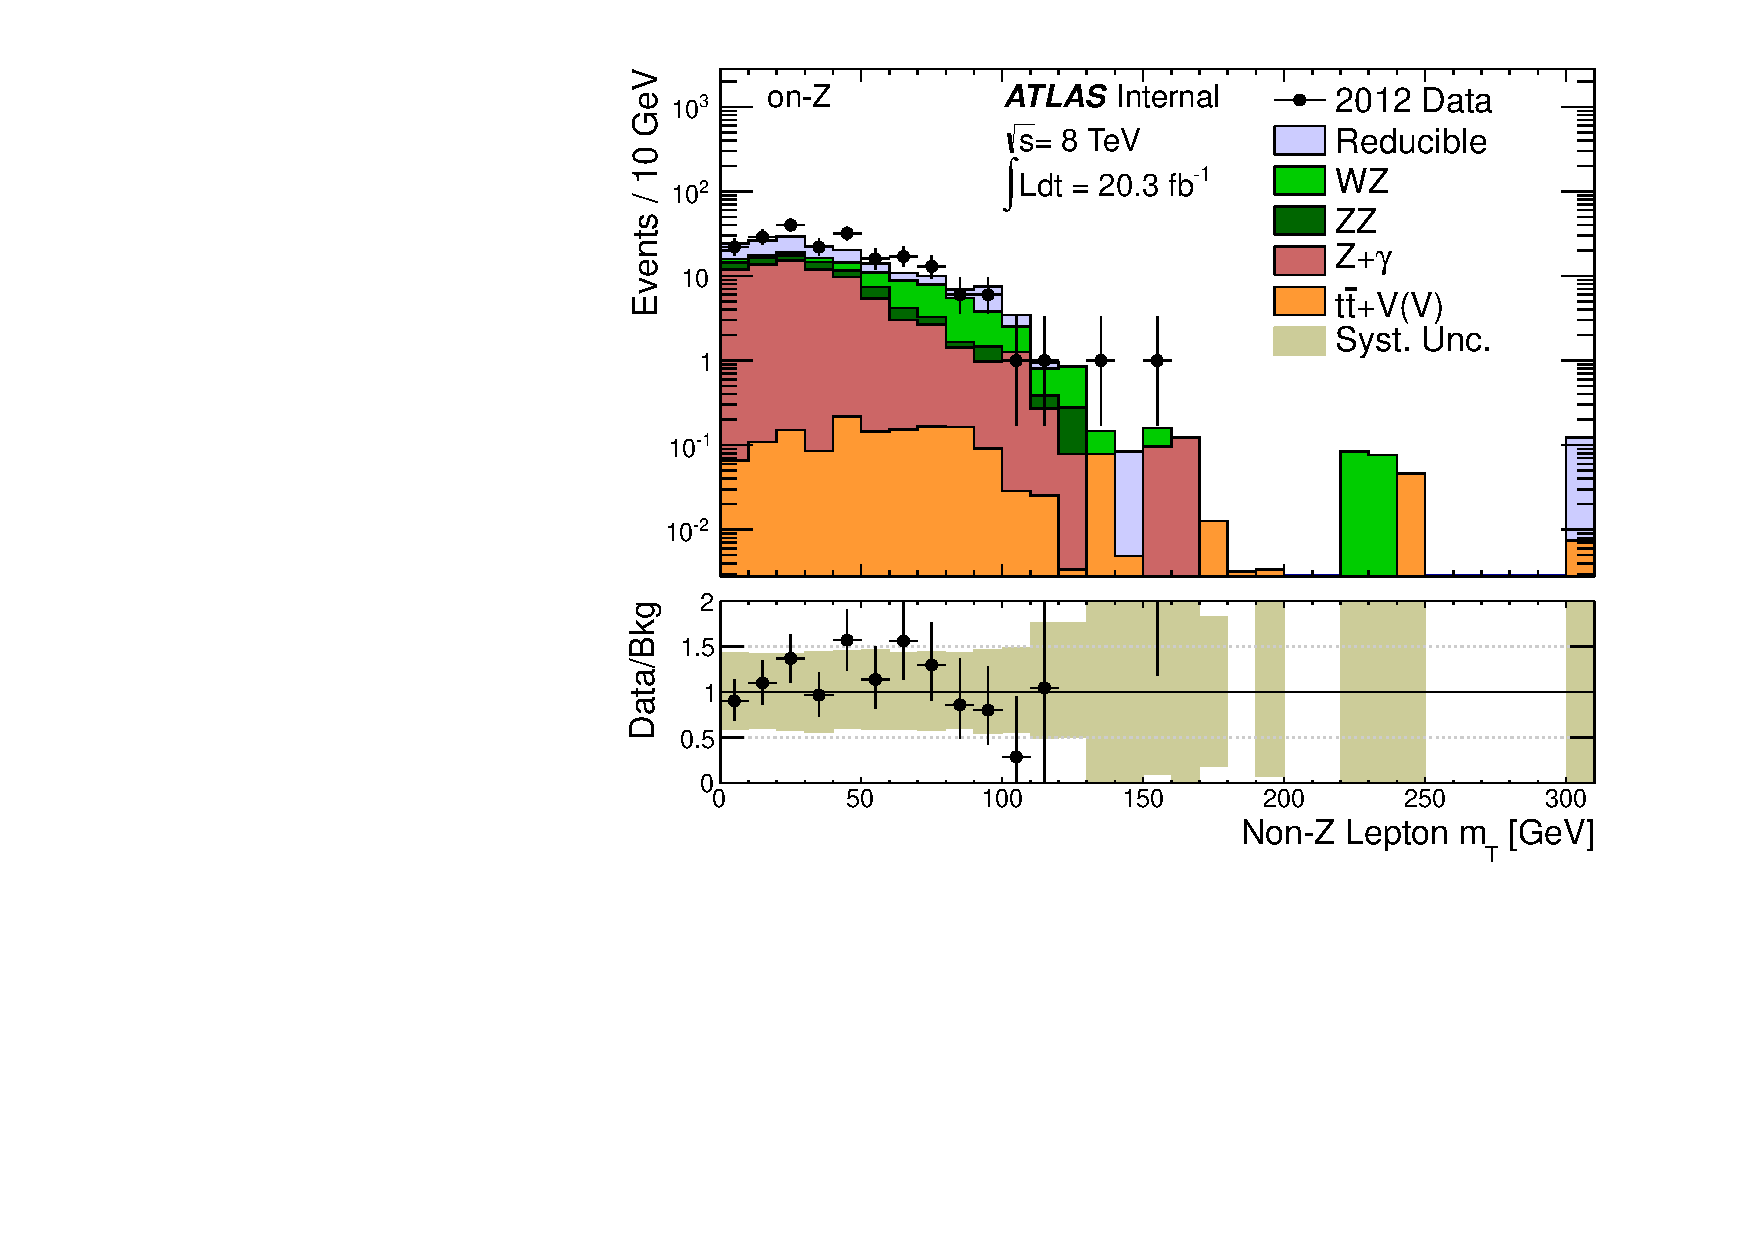
\includegraphics[width=.48\columnwidth]{figures/modelindependent/Z_emu_Zmm_offZe_intelec_OffZMT}} \\
  \subfloat[\meff]{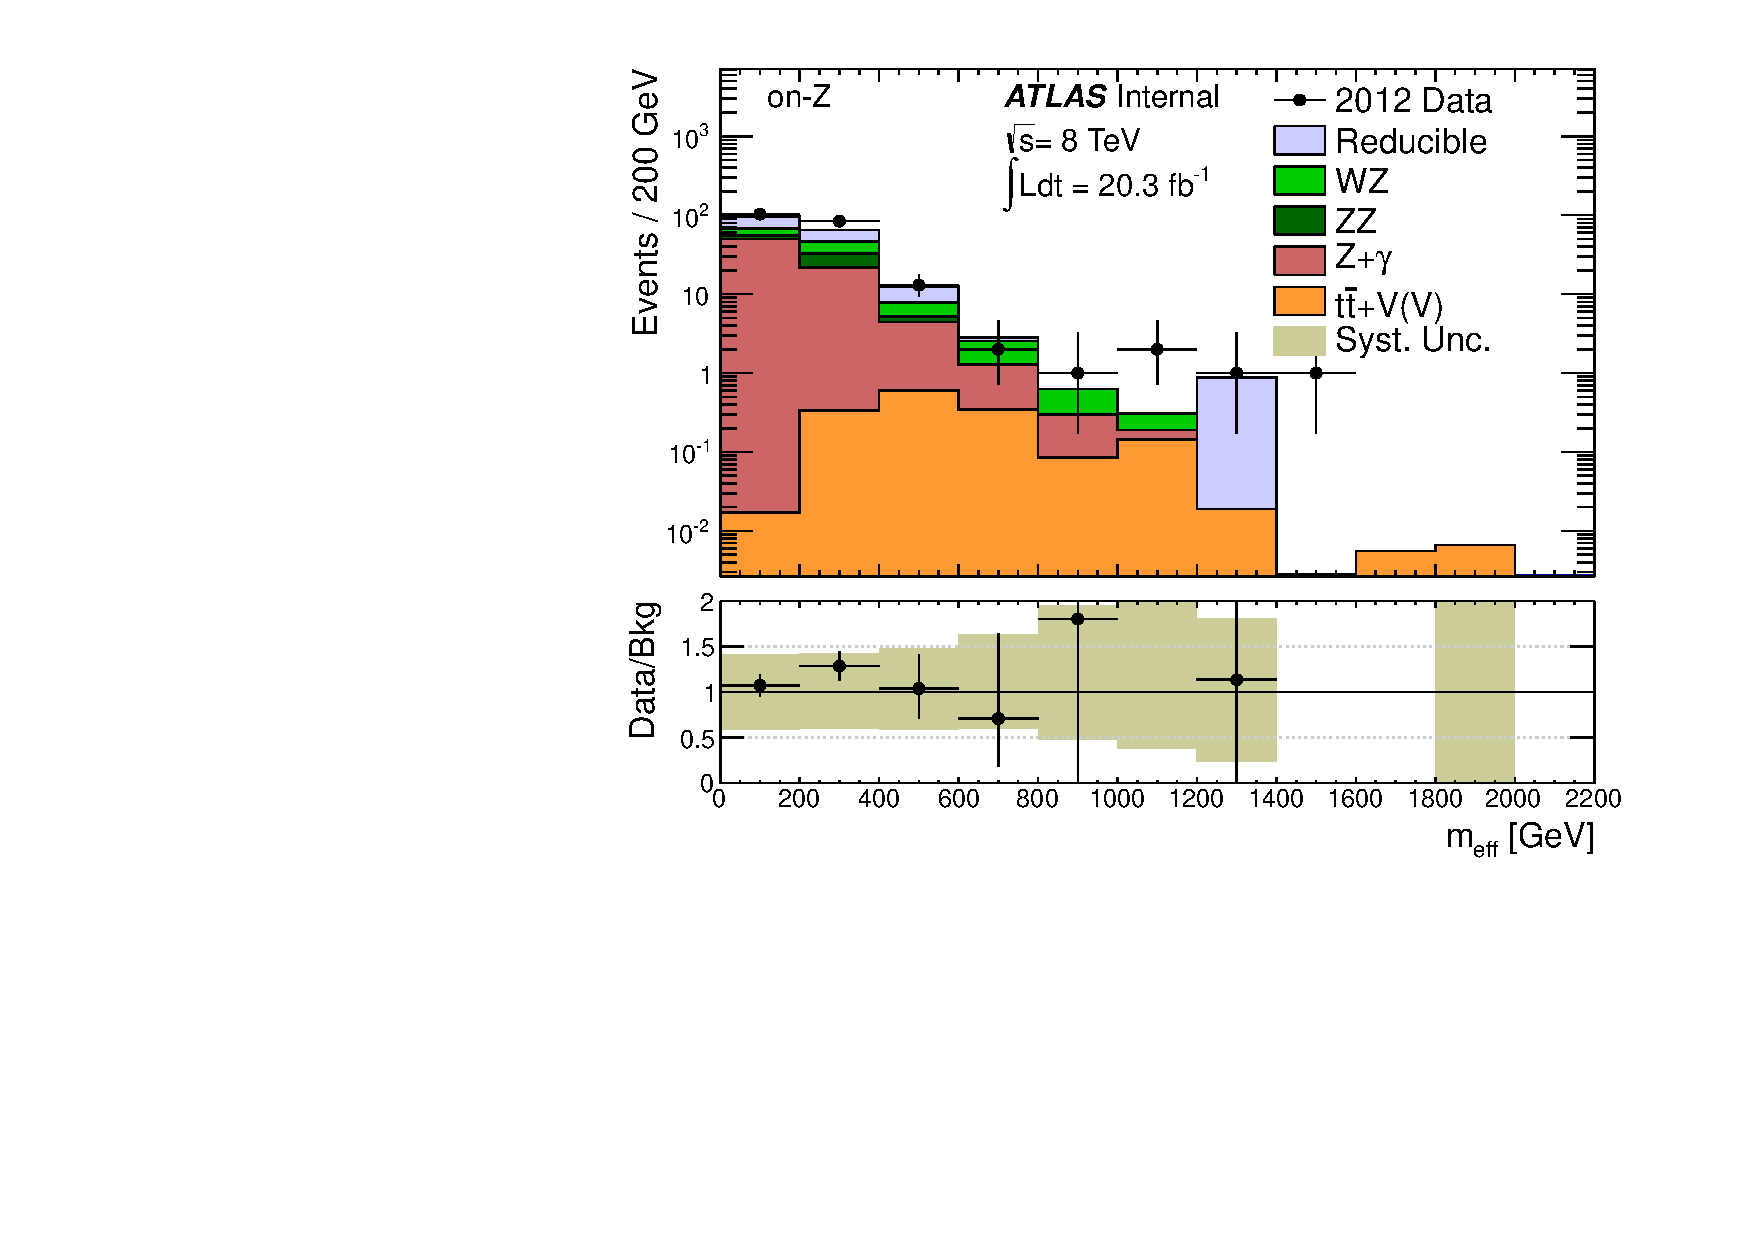
\includegraphics[width=.48\columnwidth]{figures/modelindependent/Z_emu_Zmm_offZe_intelec_ST}}
  \hfill
  \subfloat[\met]{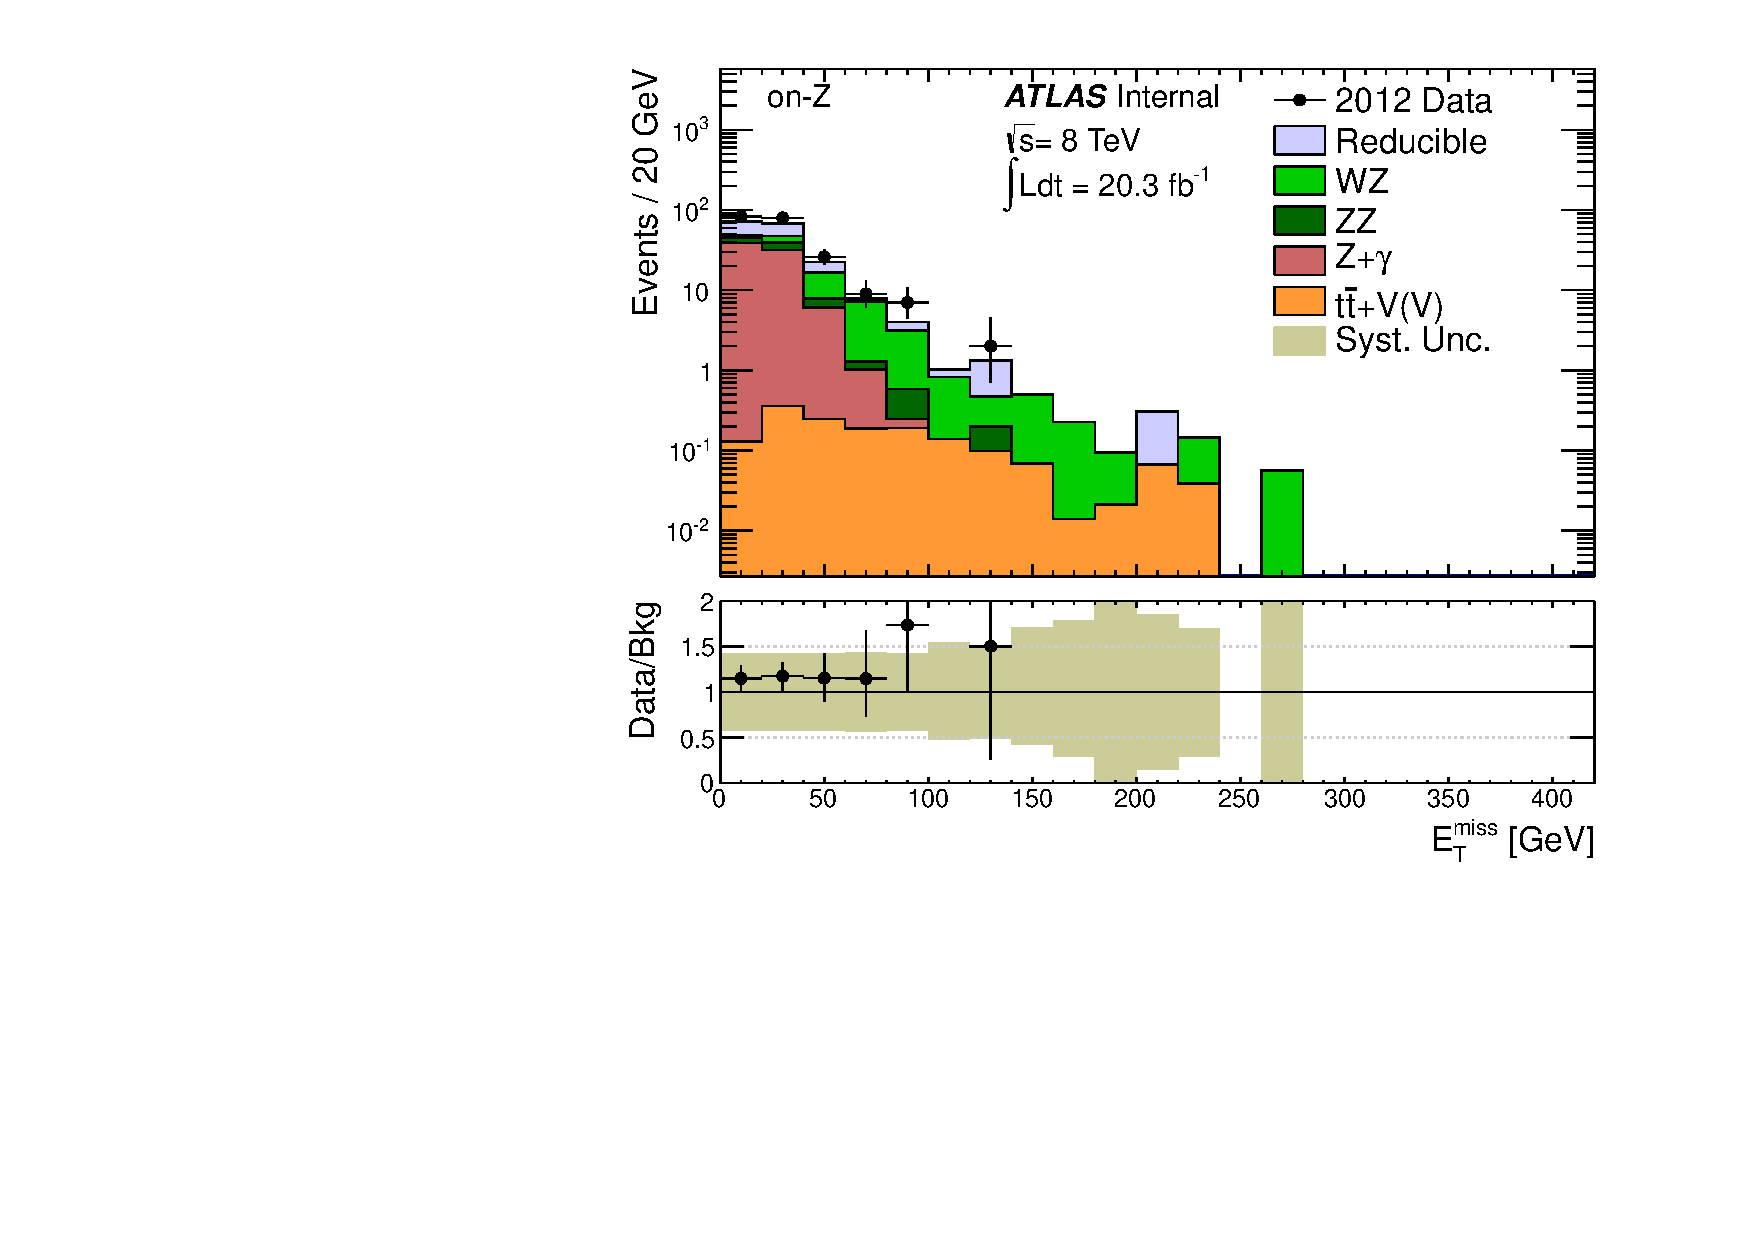
\includegraphics[width=.48\columnwidth]{figures/modelindependent/Z_emu_Zmm_offZe_intelec_MET}}
  \caption{Expected backgrounds in the intermediate-electron validation region, using the
    nominal background estimation techniques.}
  \label{fig:model-independent-VR-intermediate-e}
\end{figure}

\begin{figure}[tbp]\centering
  \subfloat[Event Composition]{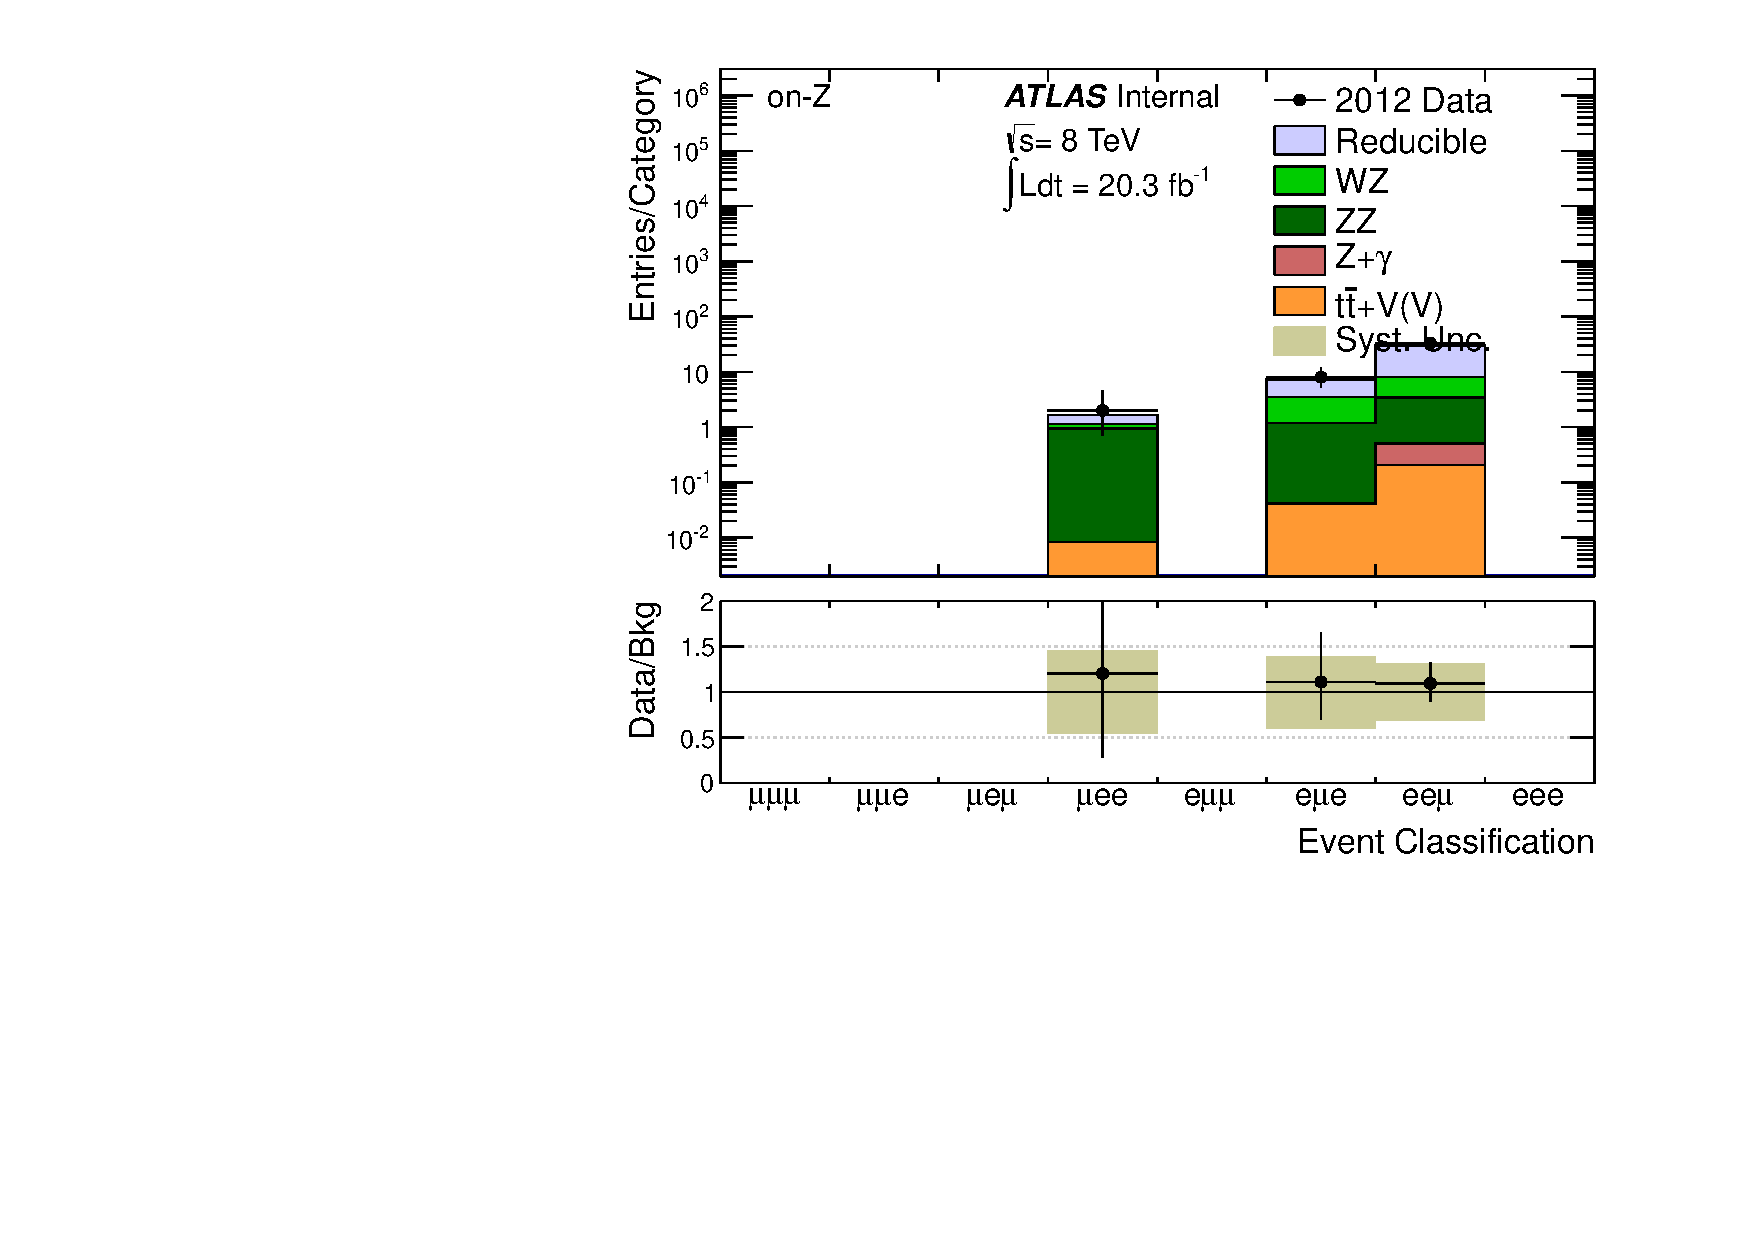
\includegraphics[width=.48\columnwidth]{figures/modelindependent/Z_emu_Zee_offZmu_intmuon_Simple3LEventClassification}}
  \hfill
  \subfloat[Muon \pt]{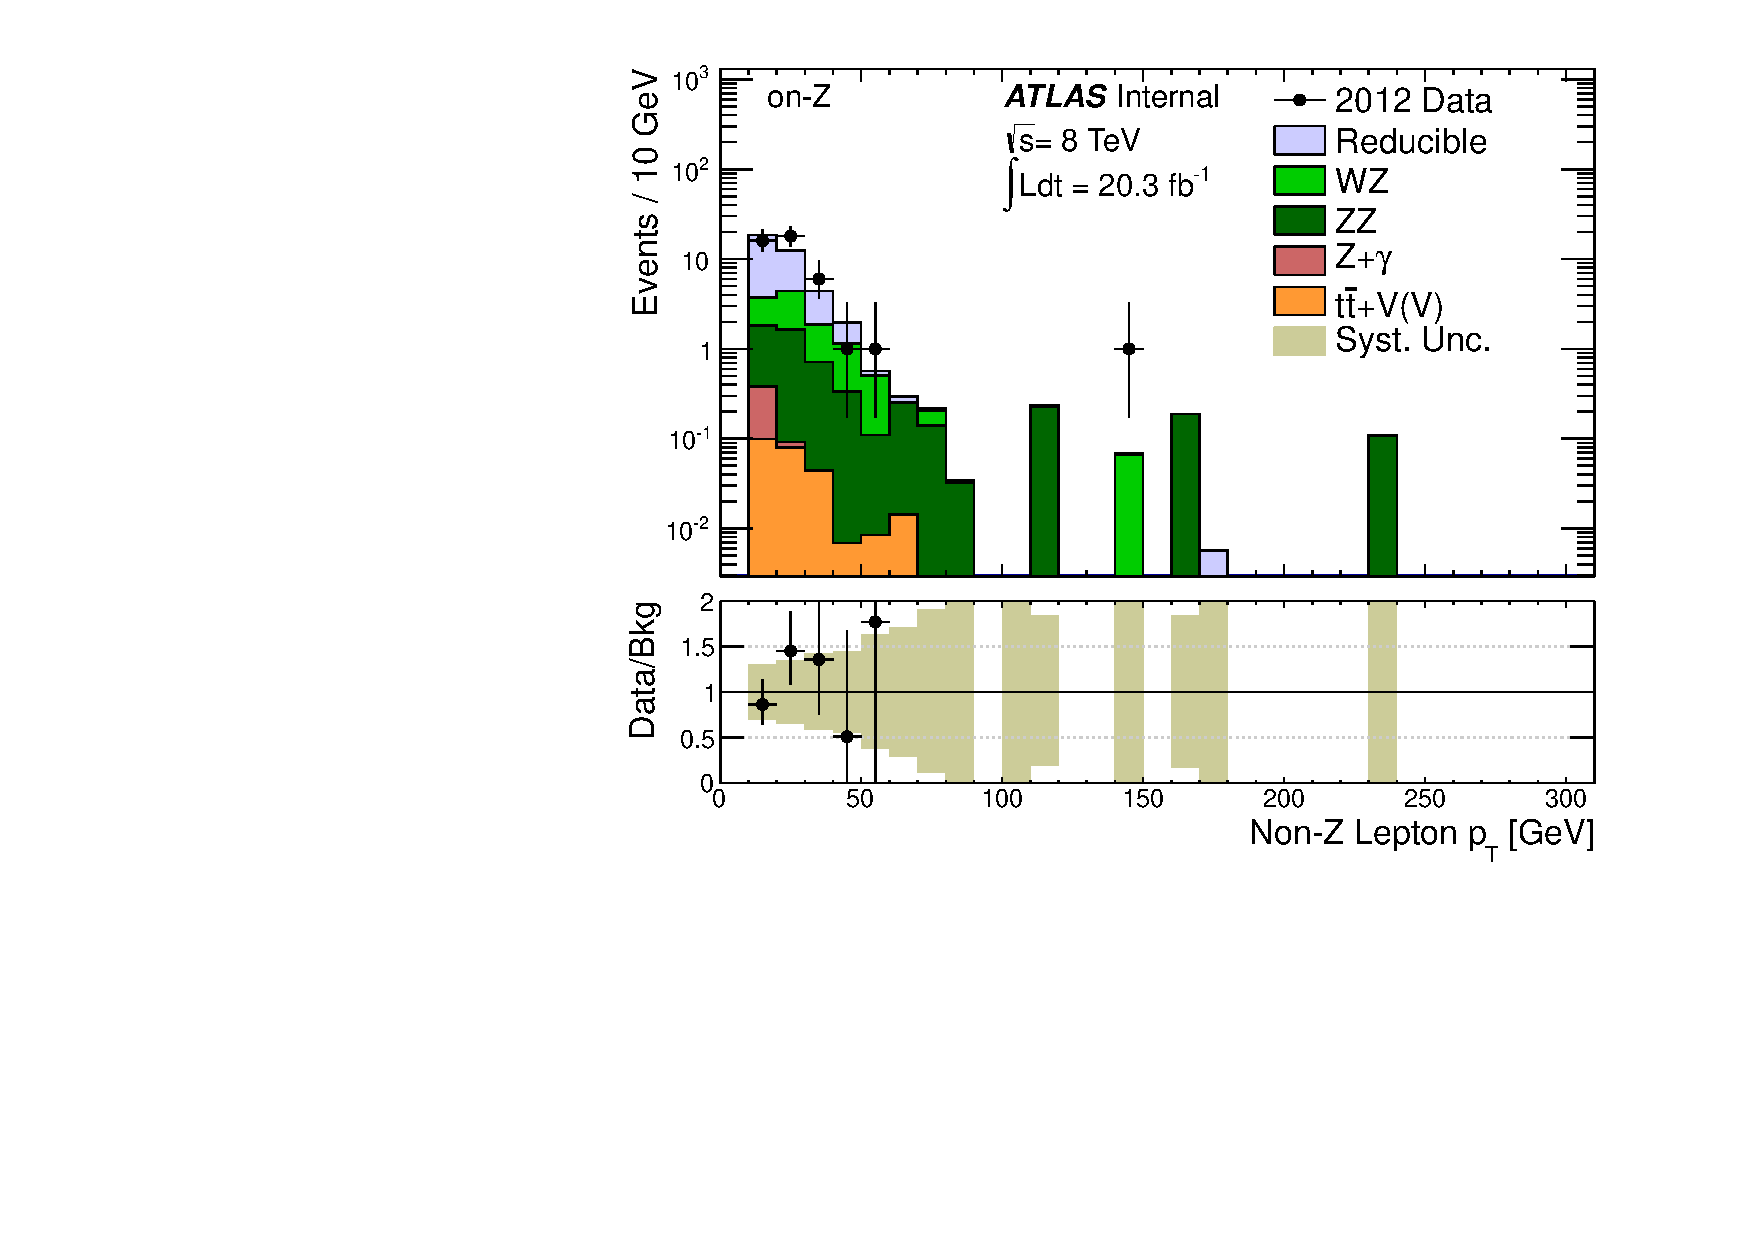
\includegraphics[width=.48\columnwidth]{figures/modelindependent/Z_emu_Zee_offZmu_intmuon_OffZPt}} \\
  \subfloat[Muon $\eta$]{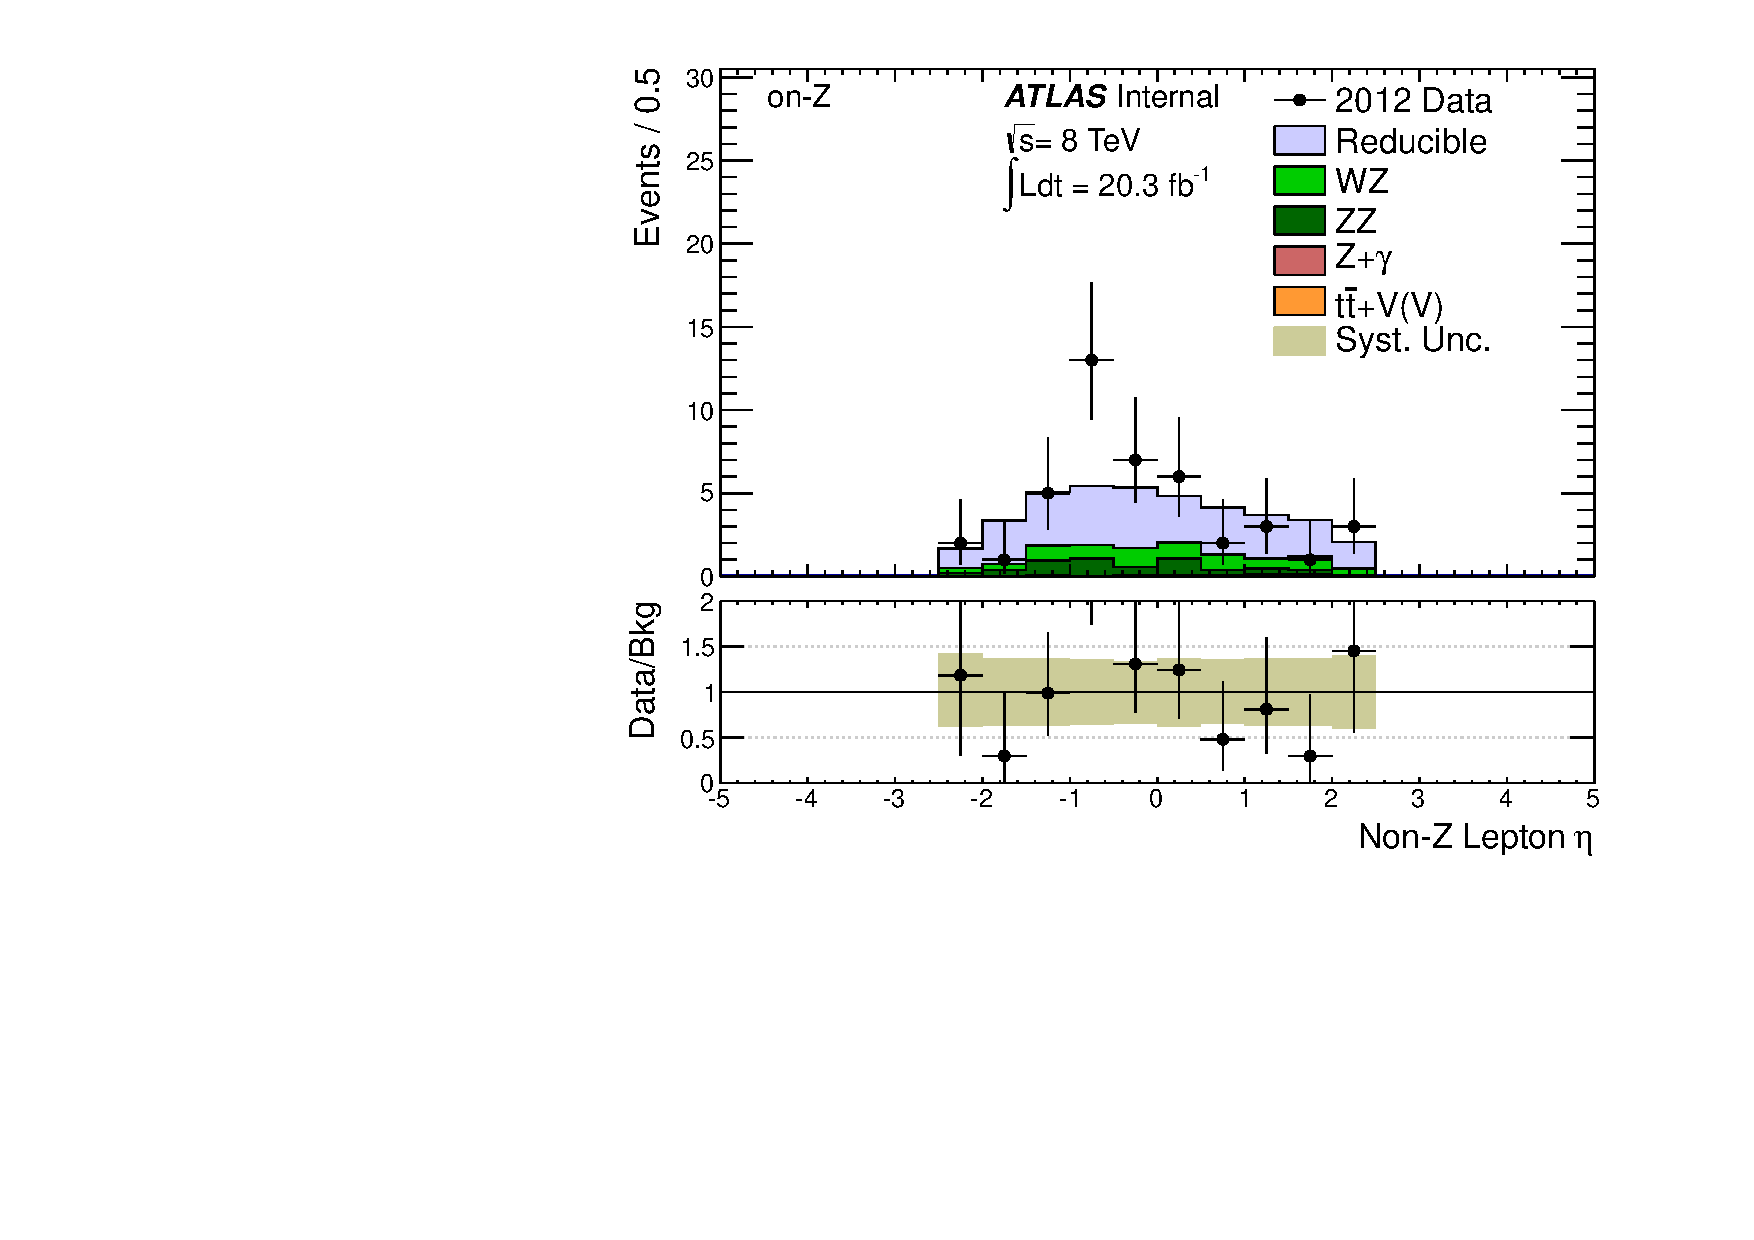
\includegraphics[width=.48\columnwidth]{figures/modelindependent/Z_emu_Zee_offZmu_intmuon_OffZEta}}
  \hfill
  \subfloat[Muon \mt]{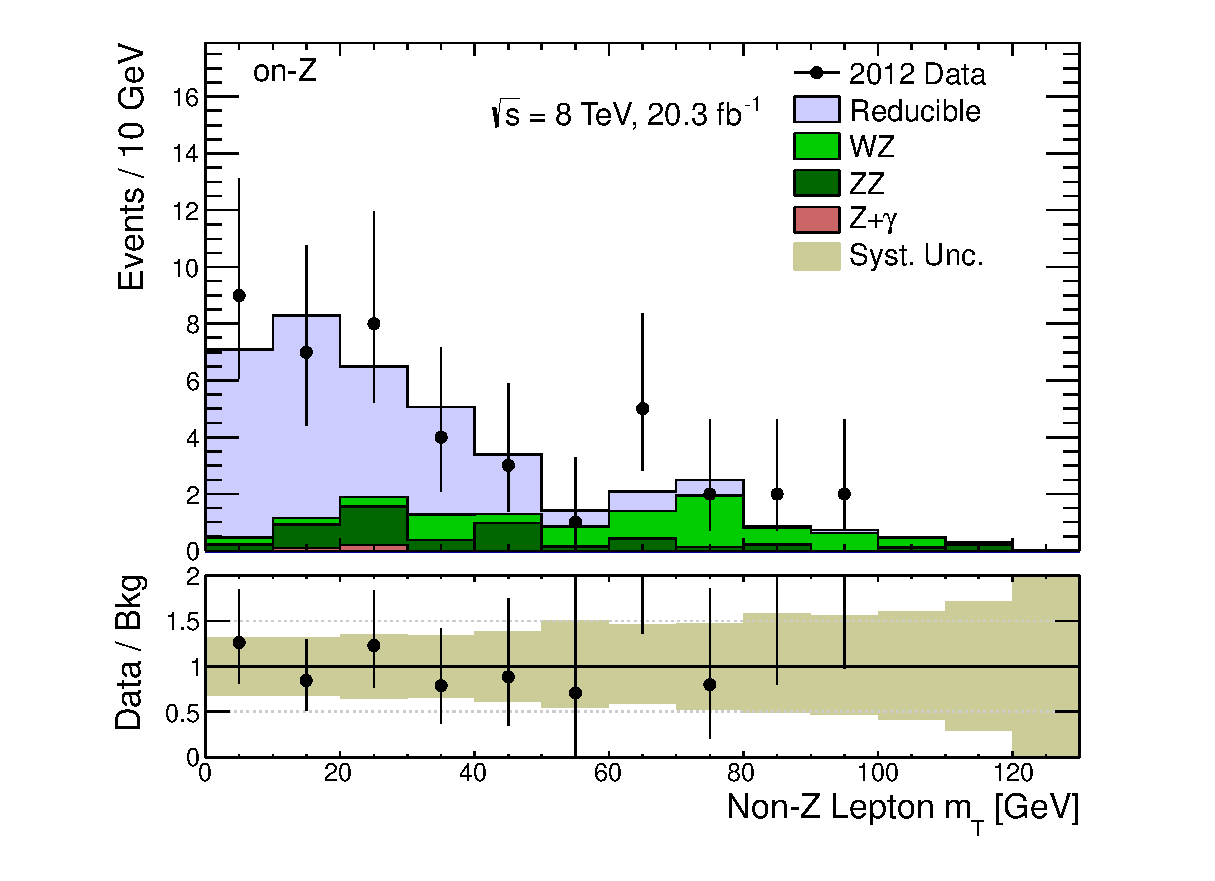
\includegraphics[width=.48\columnwidth]{figures/modelindependent/Z_emu_Zee_offZmu_intmuon_OffZMT}} \\
  \subfloat[\meff]{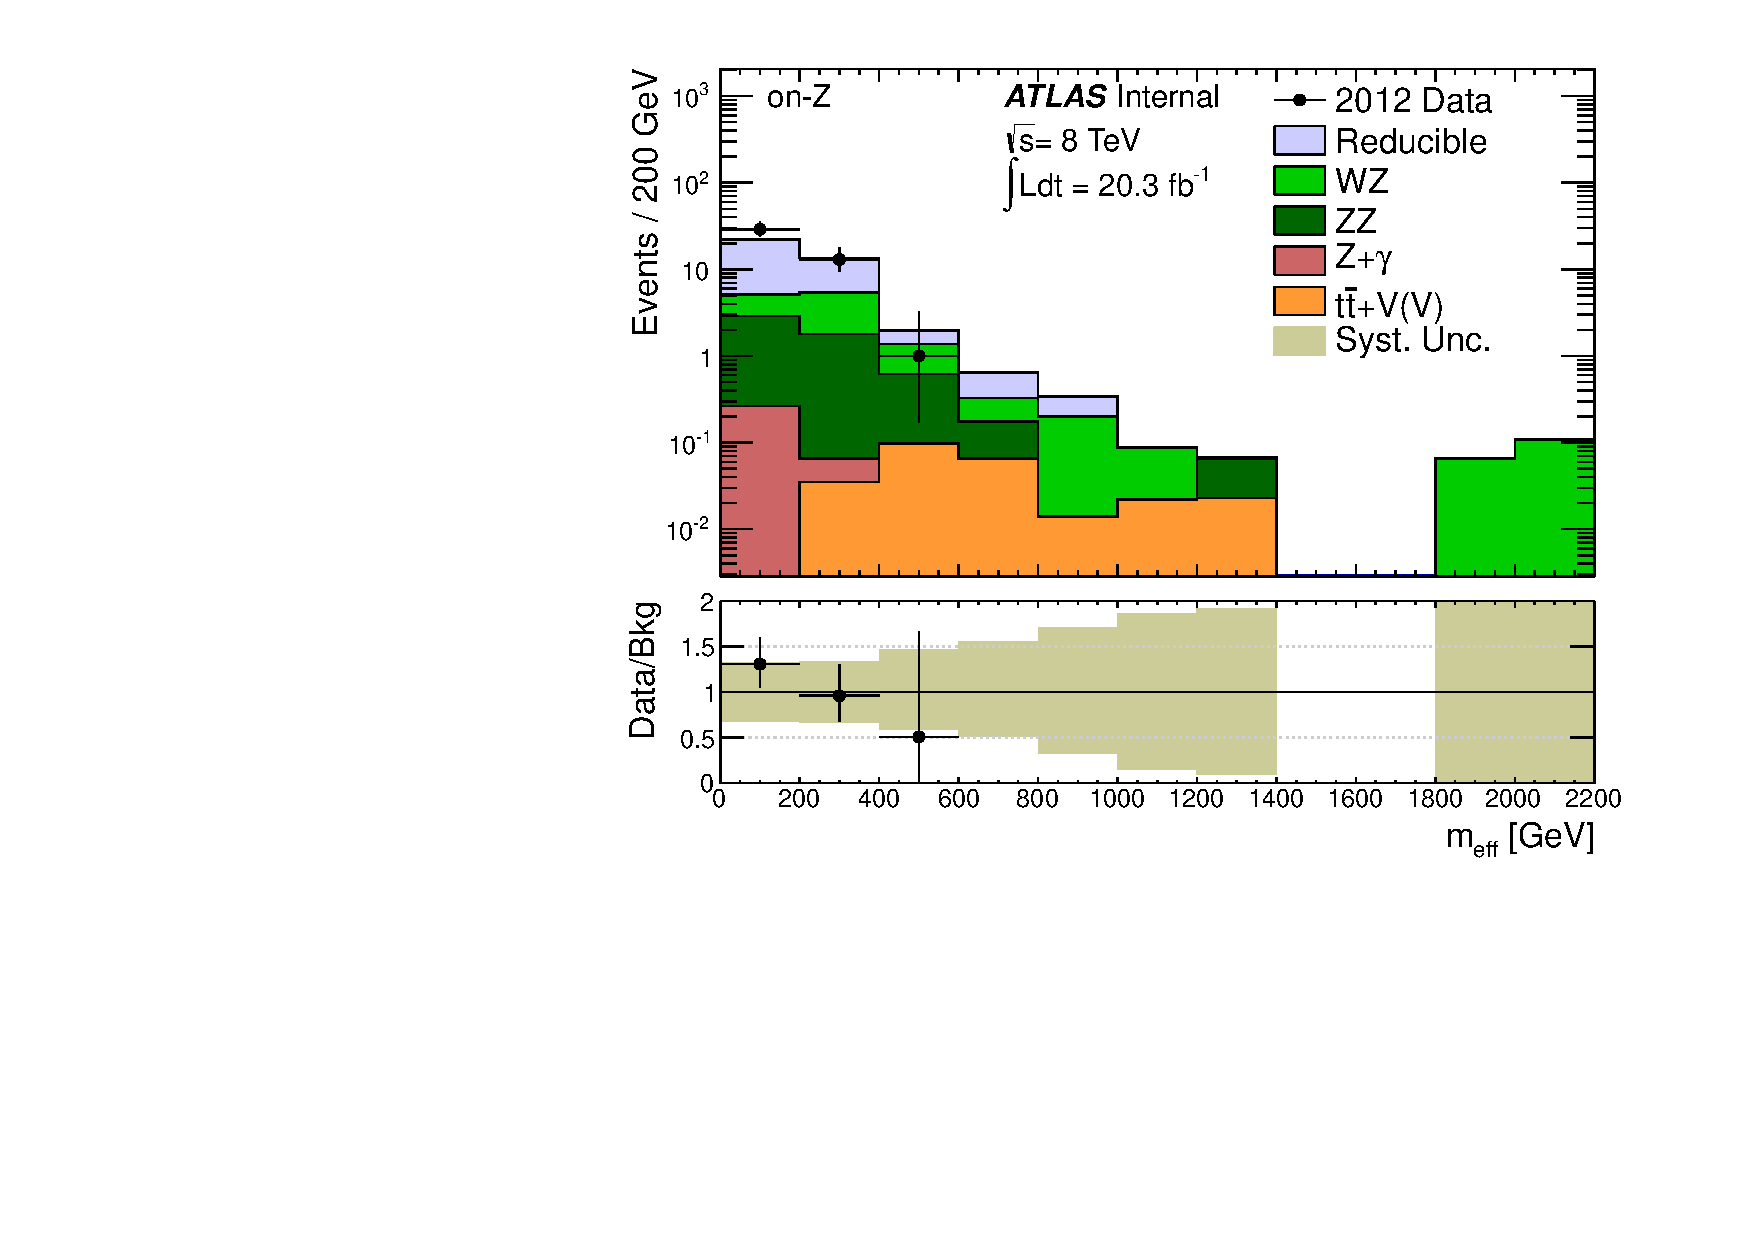
\includegraphics[width=.48\columnwidth]{figures/modelindependent/Z_emu_Zee_offZmu_intmuon_ST}}
  \hfill
  \subfloat[\met]{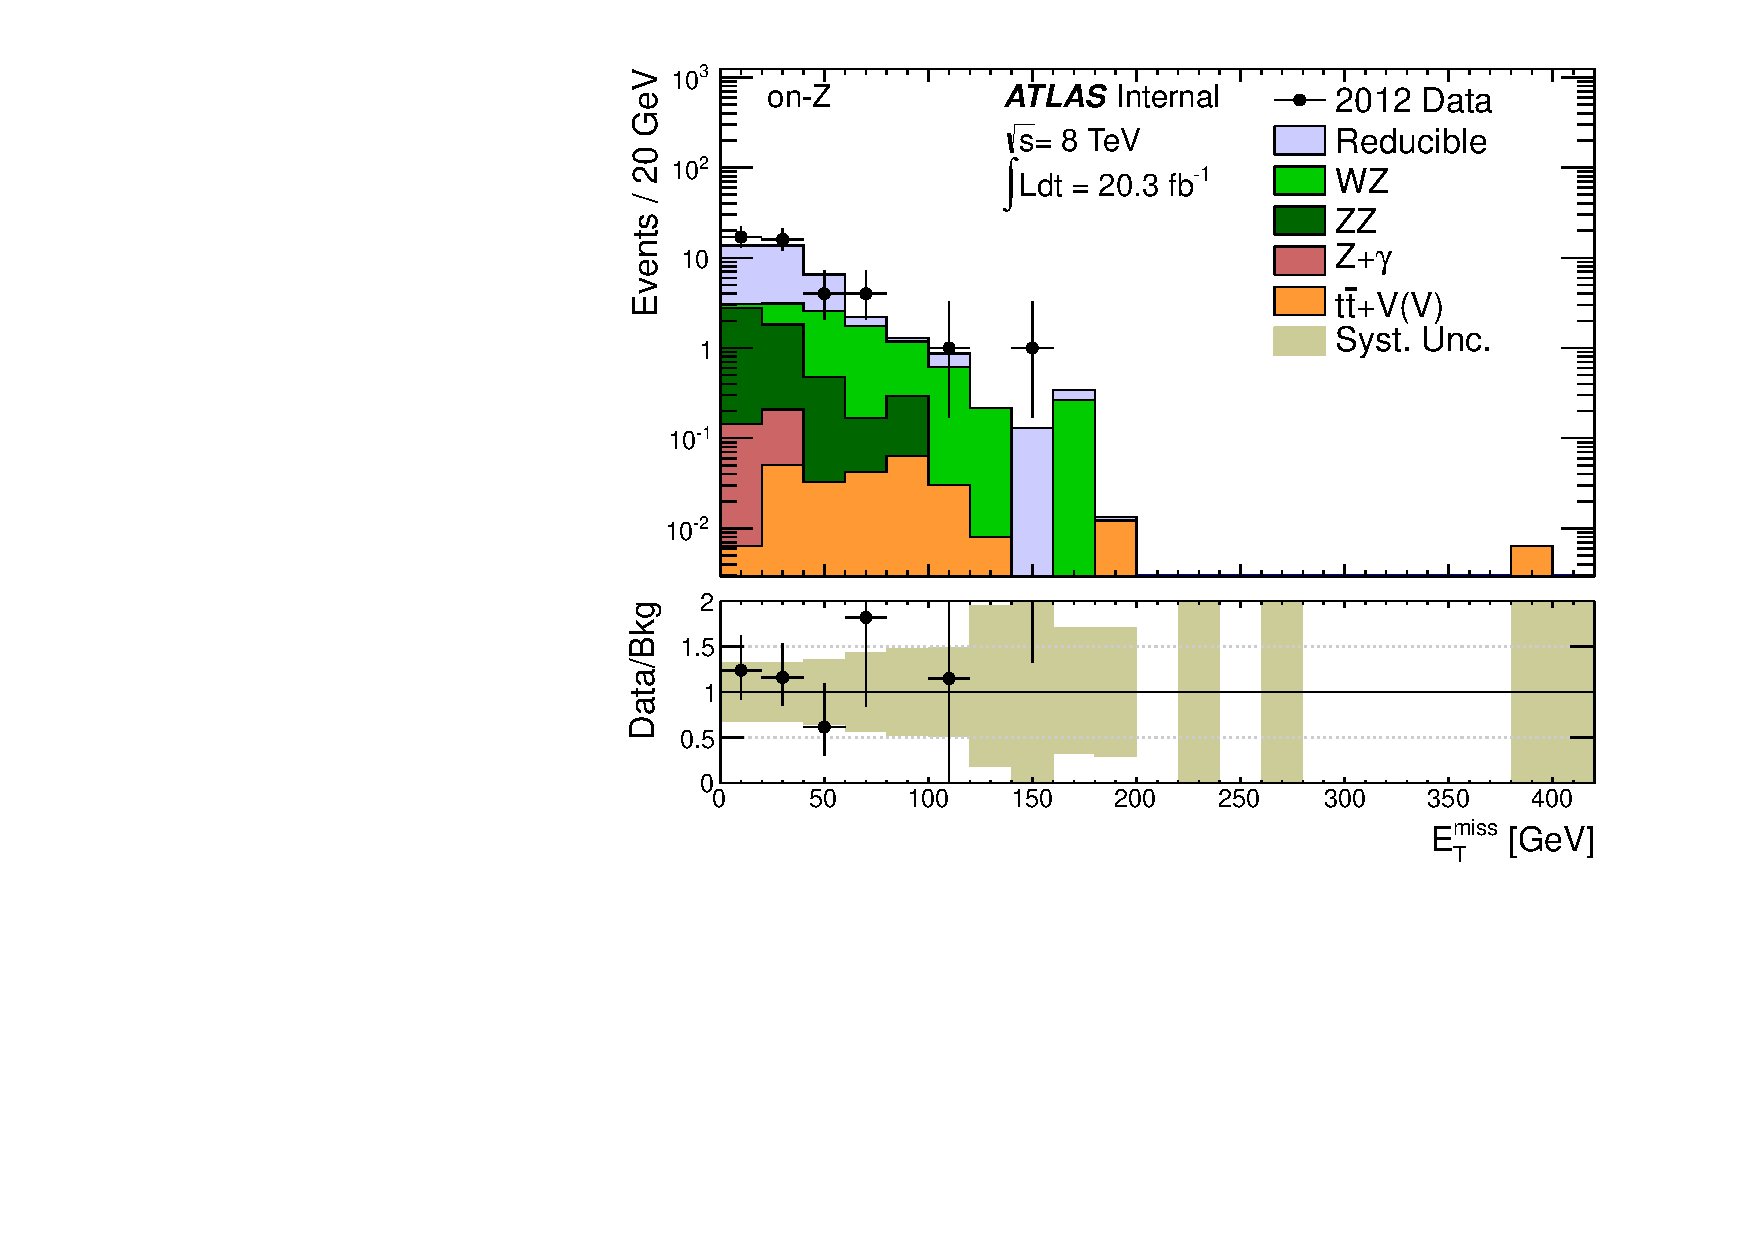
\includegraphics[width=.48\columnwidth]{figures/modelindependent/Z_emu_Zee_offZmu_intmuon_MET}}
  \caption{Expected backgrounds in the intermediate-muon validation region, using the
    nominal background estimation techniques.}
  \label{fig:model-independent-VR-intermediate-mu}
\end{figure}

The events containing an intermediate $\tau_{\mathrm{had}}$ are much more abundant than intermediate electrons or muons, so three $\tau_{\mathrm{had}}$ validation regions are defined, mirroring the signal region categories. Events are required to contain two electrons or muons plus an intermediate $\tau_{\mathrm{had}}$, and are separated into on-$Z$, off-$Z$/OSSF, and off-$Z$/mixed categories, depending on the two electrons or muons. The $\pt$ and $\eta$ of the intermediate $\tau_{\mathrm{had}}$ is shown for each category in figure~\ref{fig:model-independent-VR-intermediate-tau}.

\begin{figure}[tbp]\centering
  \subfloat[Intermediate $\tau_{\mathrm{had}}$ $p_{T}$, on-$Z$]{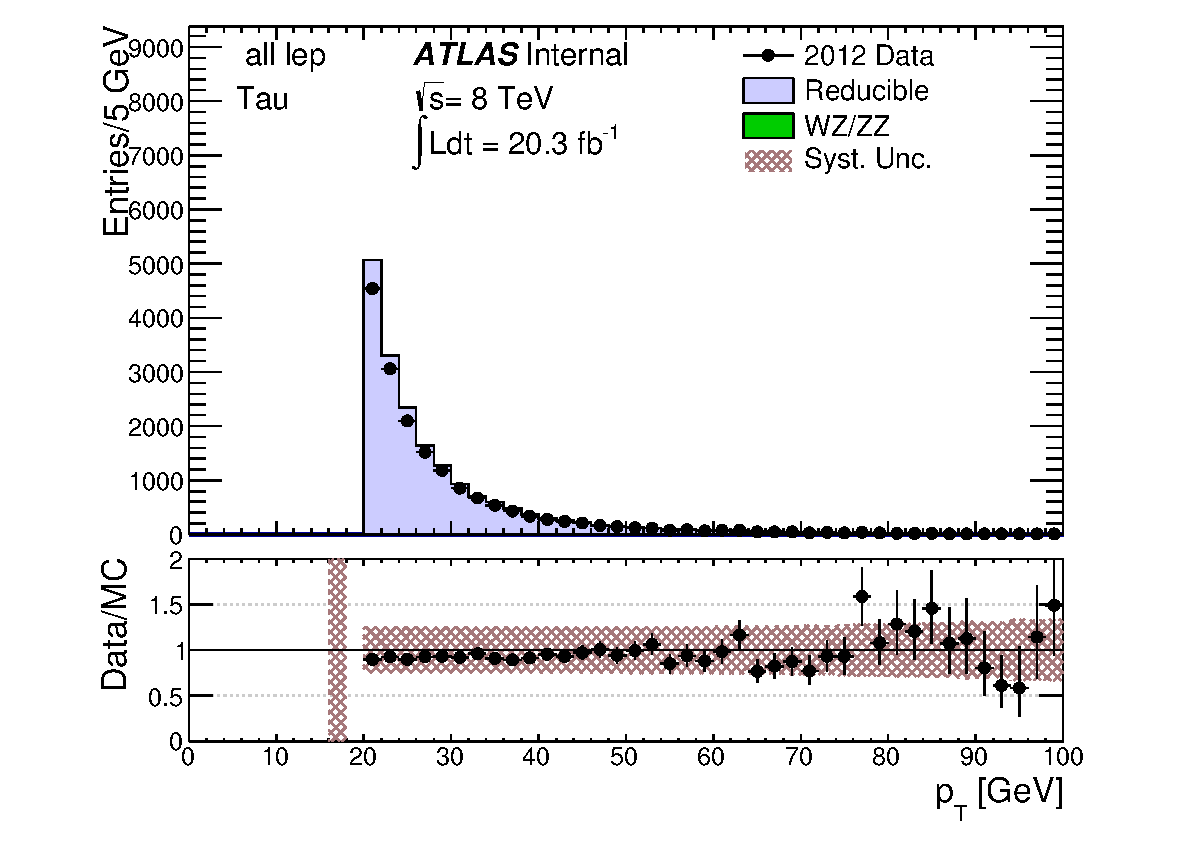
\includegraphics[width=.44\columnwidth]{figures/modelindependent/inttau_onZ_DY_TauPt}}
  \hfill
  \subfloat[Intermediate $\tau_{\mathrm{had}}$ $\eta$, on-$Z$]{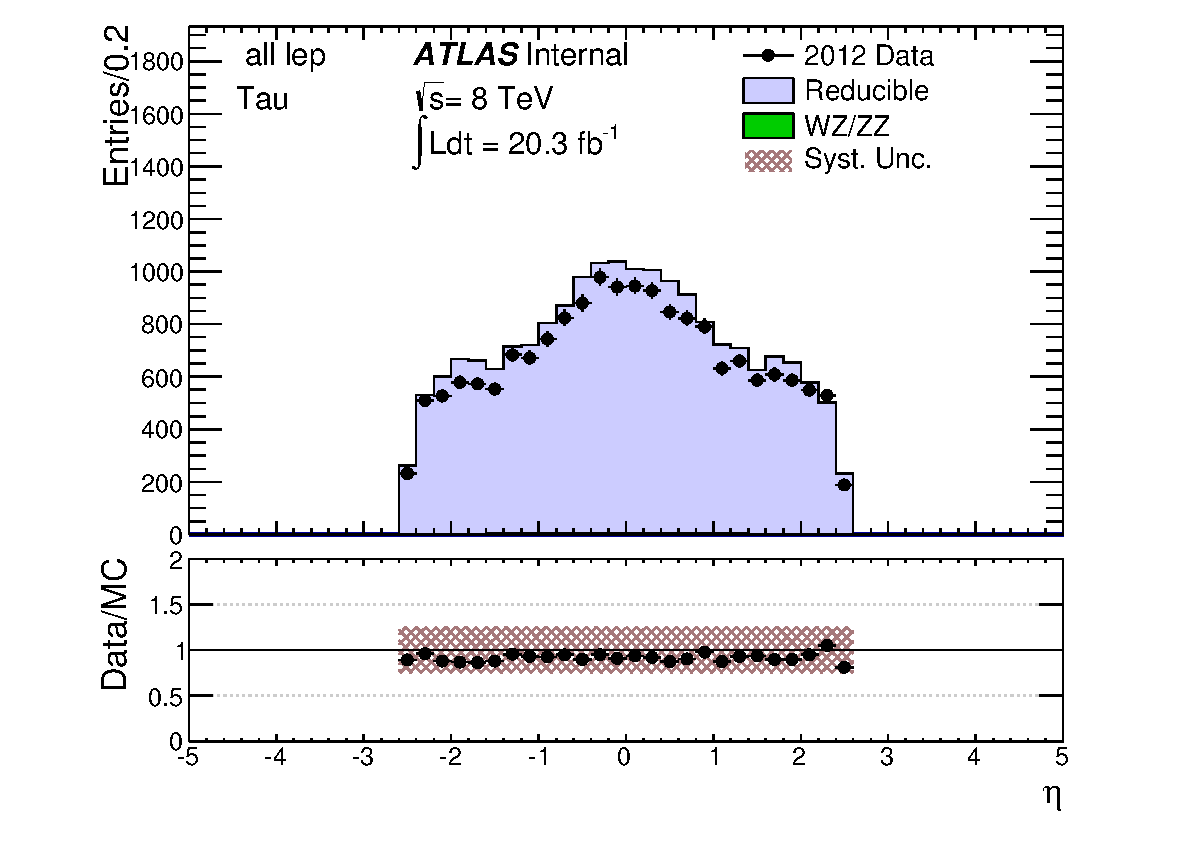
\includegraphics[width=.44\columnwidth]{figures/modelindependent/inttau_onZ_DY_TauEta}} \\
  \subfloat[Intermediate $\tau_{\mathrm{had}}$ $p_{T}$, off-$Z$/OSSF]{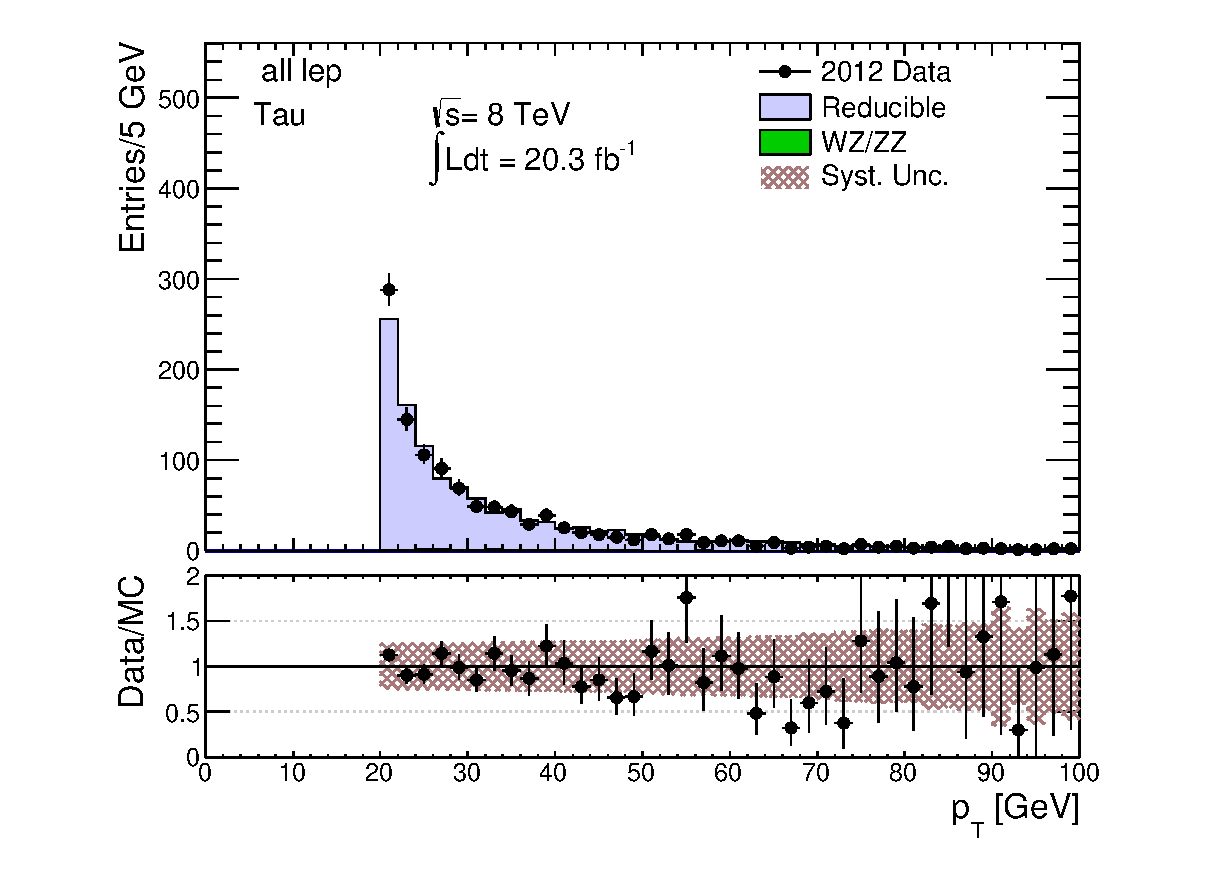
\includegraphics[width=.44\columnwidth]{figures/modelindependent/inttau_offZ_OSSF_DY_TauPt}}
  \hfill
  \subfloat[Intermediate $\tau_{\mathrm{had}}$ $\eta$, off-$Z$/OSSF]{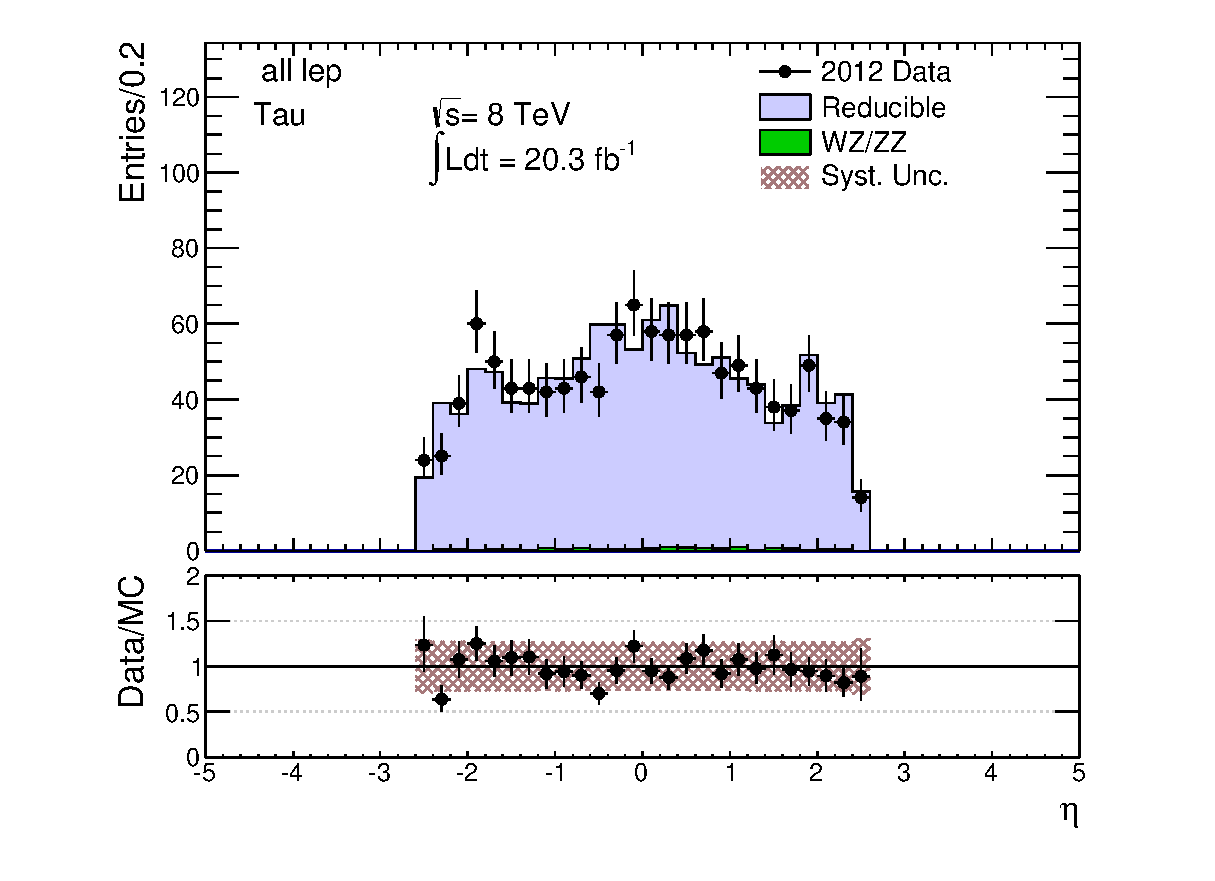
\includegraphics[width=.44\columnwidth]{figures/modelindependent/inttau_offZ_OSSF_DY_TauEta}} \\
  \subfloat[Intermediate $\tau_{\mathrm{had}}$ $p_{T}$, off-$Z$/mixed]{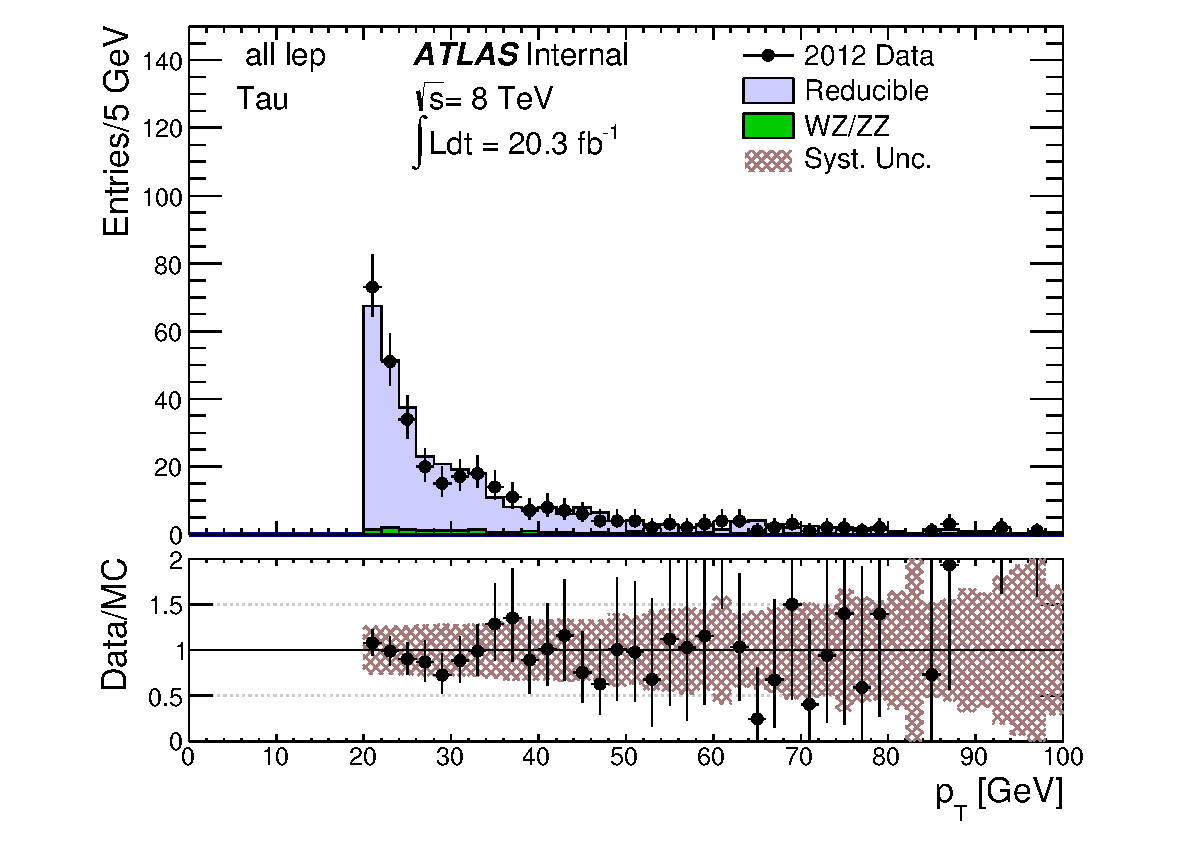
\includegraphics[width=.44\columnwidth]{figures/modelindependent/inttau_offZ_mixed_DY_TauPt}}
  \hfill
  \subfloat[Intermediate $\tau_{\mathrm{had}}$ $\eta$, off-$Z$/mixed]{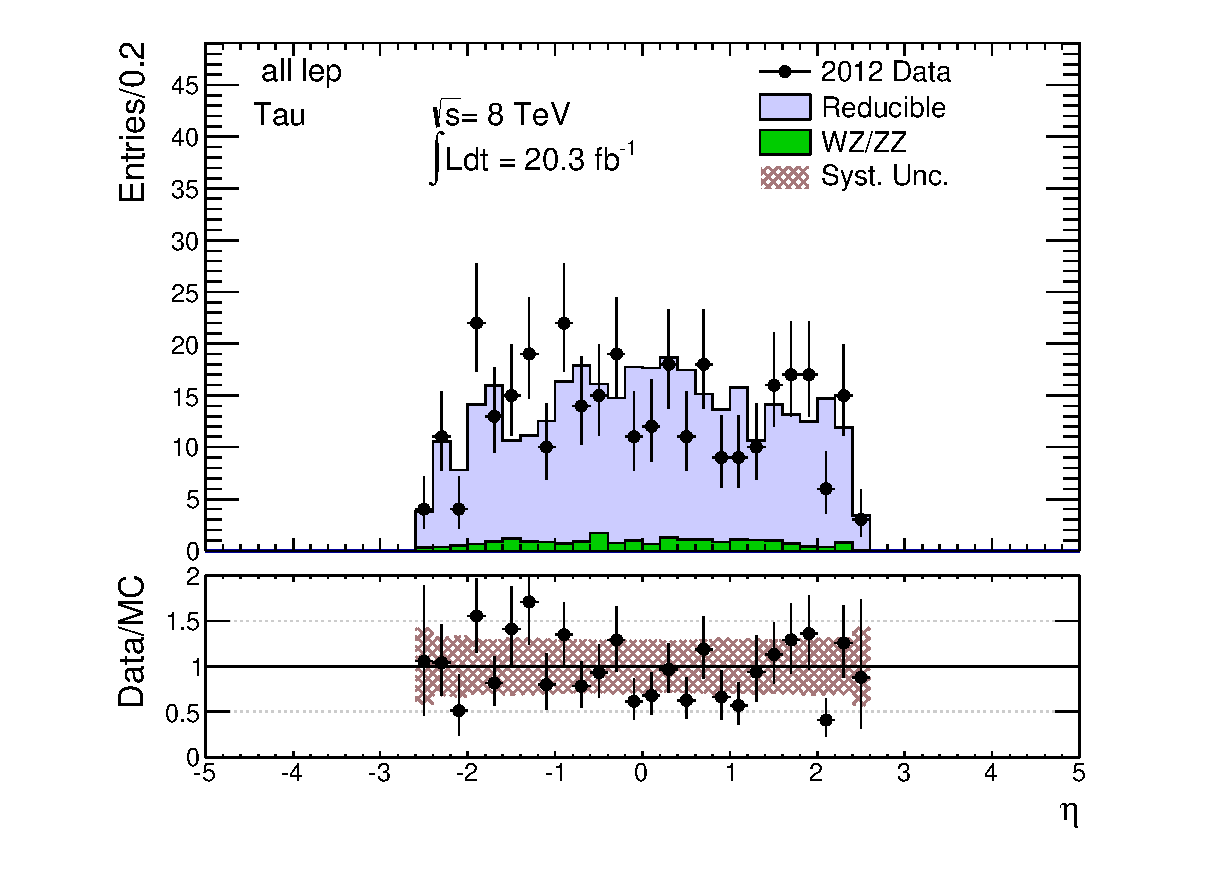
\includegraphics[width=.44\columnwidth]{figures/modelindependent/inttau_offZ_mixed_DY_TauEta}} \\
  \caption{$\pt$ and $\eta$ distributions of the intermediate $\tau_{\mathrm{had}}$ in the on-$Z$, off-$Z$/OSSF, and off-$Z$/mixed intermediate validation regions. }
  \label{fig:model-independent-VR-intermediate-tau}
\end{figure}


\section{Results and Limits}\label{sec:model-independent-results}
The results of the search as organized as follows. For each category, the distributions of the various kinematic variables ($\htlep$, $\htjets$, $\meff$, $\Etmiss$, $\mtw$, $N_{\mathrm{jets}}$, $N_{b-\mathrm{tags}}$, and the $\pt$ of the third lepton) are produced (where applicable). Then, in each of the 138 signal regions, the number of observed and expected events are compared, and, absent any significant deviations, $95\%$ confidence level (CL) upper limits are derived on the number of events from new physics, $N_{95}$, and the corresponding \emph{visible cross section}, $\sigma_{95}^{\mathrm{vis}}$, defined as

\begin{equation}
	\sigma_{95}^{\mathrm{vis}} = \frac{N_{95}}{\mathcal{L}},
\end{equation}

where $\mathcal{L}=20.3~\mbox{fb}^{-1}$ is the integrated luminosity of the data.

The plots for the $\htlep$ signal regions are shown here for demonstrative purposes. The full set of plots is available at~\cite{model-independent-webpage}. The $\htlep$ distributions are shown in figure~\ref{fig:model-independent-htlep}. The observed and expected event counts in the three corresponding signal regions ($\htlep>200 \GeV$, $\htlep>500 \GeV$, and $\htlep>800 \GeV$) are shown in table~\ref{table:model-independent-htlep}. Finally, the upper limits on $\sigma_{95}^{\mathrm{vis}}$ are shown in figure~\ref{fig:model-independent-htlep-sigmavis}. 

The deviations between the observed and expected in all 138 signal regions are shown in figure~\ref{fig:model-independent-summary-sigma}, in units of the total uncertainty on the background expectation. 

\begin{figure}[htbp]
	\centering

	\caption{$\htlep$ distributions in the six categories.}
	\label{fig:model-independent-htlep}
\end{figure}

\begin{table}[htbp]
	\centering

	\caption{Observed and expected event counts in the $\htlep$ signal regions, along with the inclusive counts for the entire category.}
	\label{table:model-independent-htlep}
\end{table}

\begin{figure}
	\centering

	\caption{95\% CL upper limits on the visible cross section of trilepton event production from new physics, $\sigma_{95}^{\mathrm{vis}}$, in each $\htlep$ signal region. }
	\label{fig:model-independent-htlep-sigmavis}
\end{figure}

\begin{figure}
	\centering

	\caption{Deviations between the observed event counts and the background expectations in each signal region, in units of the total uncertainty on the background prediction.}
	\label{fig:model-independent-summary-sigma}
\end{figure}



\section{Interpretations}
The 95\% CL upper limits on trilepton event production from new physics derived in section~\ref{sec:model-independent-results} provide a useful tool with which to confront models of new physics producing trilepton final states. In order to compare the predictions of a model, i.e. a set of simulated events at \textcolor{red}{particle level} from an event generator, per-lepton fiducial efficiencies are provided to quantify approximately the efficiency of reconstructing and selecting fiducial leptons at truth level. The definition of fiducial truth leptons is as follows: 

\begin{itemize}
	\item \underline{\textbf{Transverse momentum}}: Electrons and muons are required to have $\pt>10 \GeV$, while tau leptons are required to have $\pt>15 \GeV$.
	\item \underline{\textbf{Pseudorapidity}}: The same pseudorapidity cuts as the reconstructed signal leptons are applied. Electrons must have $|\eta|<2.47$, excluding the region $1.37<|\eta|<1.52$, and muons and tau leptons must have $|\eta|<2.5$.
	\item \underline{\textbf{Isolation}}: For electrons and muons, the sum of the transverse momenta of all charged particles with $\pt>1 \GeV$ within a cone of radius $\Delta R=0.3$ of the lepton, denoted \texttt{truth\_ptcone30}, must satisfy \texttt{truth\_ptcone30}/$\pt<0.15$. Similarly, the \texttt{truth\_Etcone30}, defined as the sum of all stable, visible particles within a cone of radius $\Delta R=0.3$, is required to satisfy \texttt{truth\_Etcone30}$/\pt<0.15$.
	\item \underline{\textbf{Origin and Decay}}: Leptons must originate from the hard scattering interaction (as opposed to the interaction with the detector as simulated by \geant), and not arise from the decay of a hadron. Electrons and muons are also required to be stable; tau leptons are required to decay hadronically. 
\end{itemize}

The efficiencies are derived from a Monte Carlo simulation sample 

\textcolor{red}{Efficiencies. Doubly charged higgs interpretation?}

\printbibliography